\documentclass[dvipdfmx]{beamer}
\documentclass[dvipdfmx]{beamer}
\input
\usetheme{Madrid}

\title{Current Status}
\author{Kentaro Inoue}
\date{\today}

\begin{document}
\maketitle

\begin{frame}{Items}
  \begin{itemize}
  \item Scaling factors
    \begin{itemize}
    \item Trigger and DAQ page.\pageref{page:Trig} 
    \item Beam Line Analysis (Number of kaon) page.\pageref{page:BL}
    \end{itemize}
  \item Detector performance
    \begin{itemize}
    \item CDS page.\pageref{page:CDS}
    \item NC page.\pageref{page:NC}
    \end{itemize}
  \end{itemize}
\end{frame}

\begin{frame}{Scaling Factor}
  \begin{itemize}
  \item Luminosity
    \begin{eqnarray*}
      L=N_{beam}N_{target}Eff_{DAQ}Eff_{Trigger}=5870 \pm 150 \\
      N_{target}=l(10cm)\times \rho (0.169g/cm^3) \times N_{A}/N_{d}\\
      N_{beam} N_{DAQ} N_{trigger} \mbox{were estimated run-by-run.}\\
    \end{eqnarray*}
  \item Neutron Efficiency\\
    $Eff_{NC}=0.317\pm 0.016$ by $K^-d\rightarrow K^0 n$ reaction (RUN62)\\
    $Overkill_{\overline{CVC\cup PC}}=0.081\pm0.007$ (RUN78)
  \item CDC efficeincy\\
    RUN68 IH and CDH was used as trigger counters $\sim 0.977\pm 0.004$\\
    RUN78 was estimated from the value that CDC layer1 was used instead of IH.
  \end{itemize}
\end{frame}


\begin{frame}
  \label{page:Trig}
  { \Huge Trigger and DAQ eff.}
\end{frame}
\begin{figure}[htbp]
  \centering
  \includegraphics[width=14cm]{pic/experiment/trigger.eps}
  \caption{
    Schematic view of trigger scheme
  }
  \label{fig:trigger}
\end{figure}


\begin{frame}
  \label{page:BL}
  { \Huge Beam Line Analysis \newline (Number of Kaon)}
\end{frame}
\begin{frame}{Kaon Number}
  \begin{tabular}{cc}
    \begin{minipage}{0.5\hsize}
      \begin{figure}
        Relative Ratio
        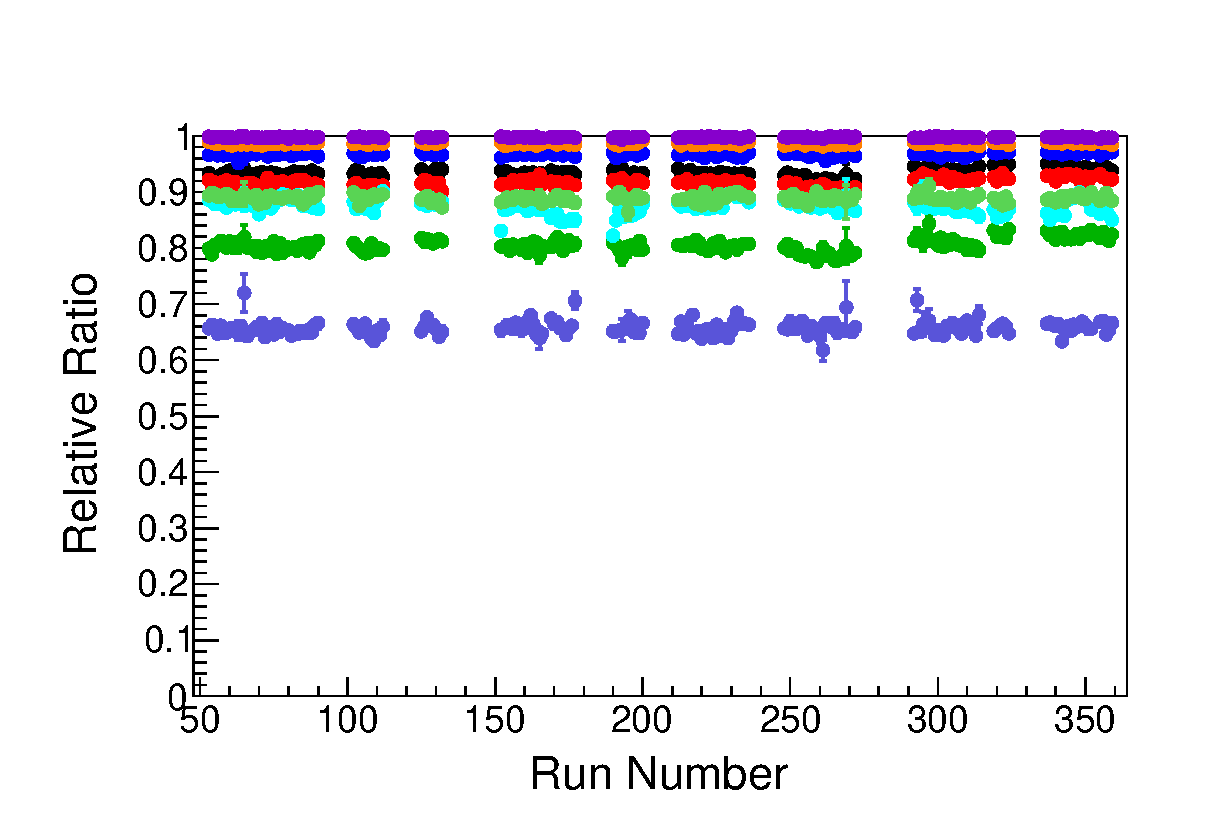
\includegraphics[width=5cm]{../pic/Run78/BL/relative_ratio.eps}
      \end{figure}
    \end{minipage}

    \begin{minipage}{0.5\hsize}
      \begin{figure}
        Survival Ratio
        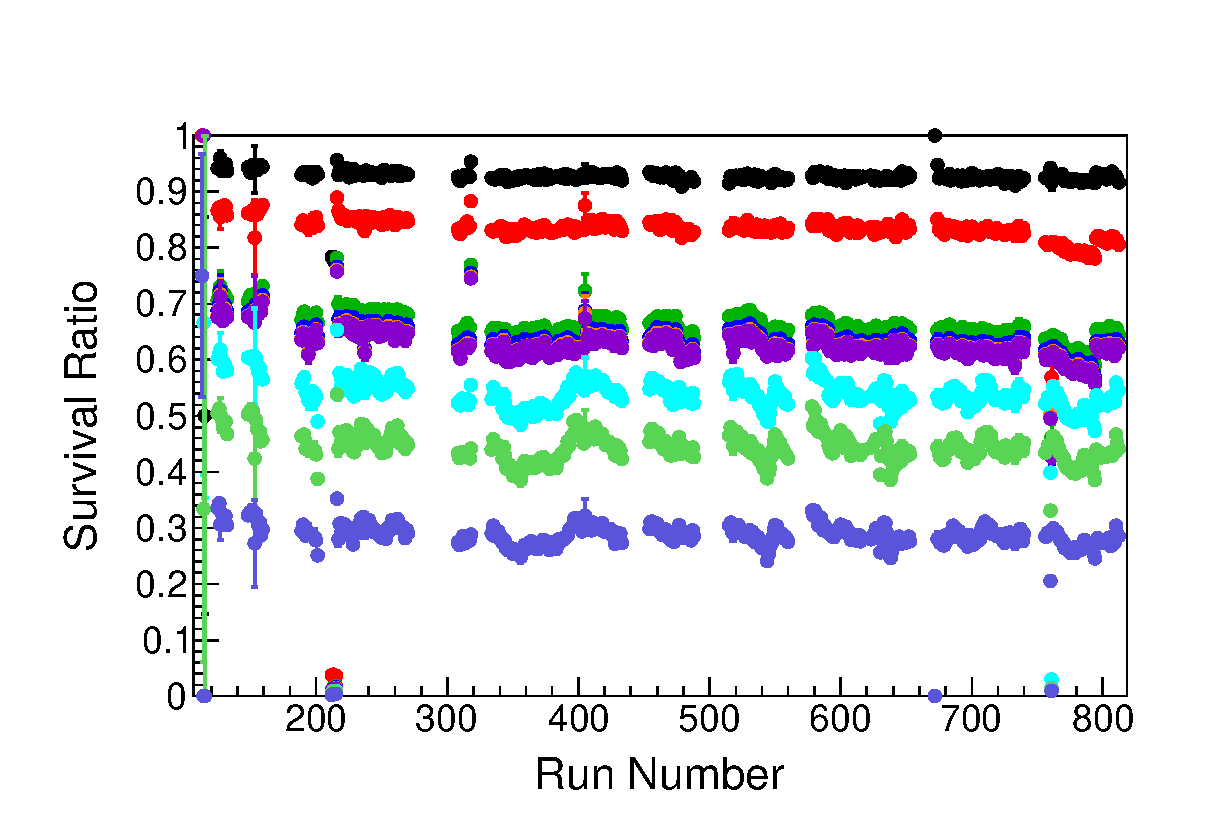
\includegraphics[width=5cm]{../pic/Run78/BL/survival_ratio.eps}
      \end{figure}
    \end{minipage}
  \end{tabular}

  \begin{tabular}{cc}
    \begin{minipage}{0.5\hsize}
      \begin{figure}
        Irradiated Kaon Number
        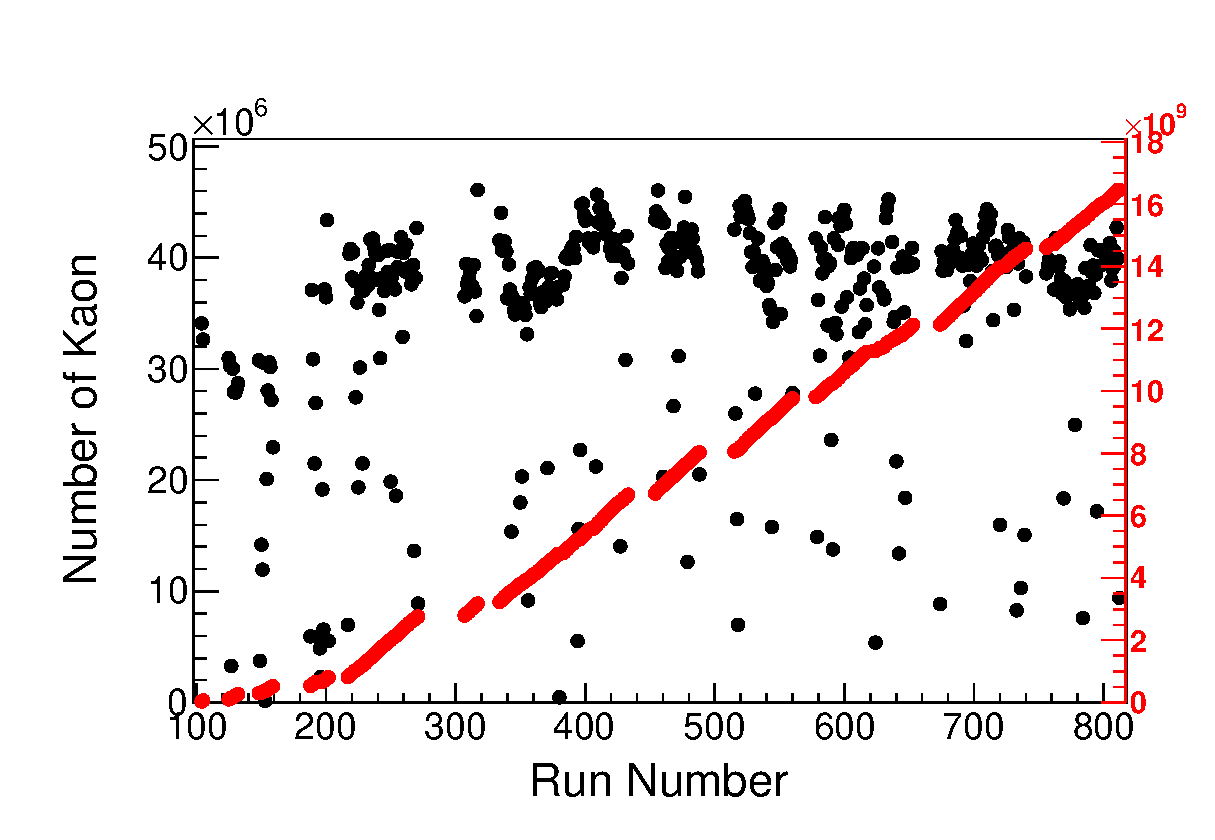
\includegraphics[width=5cm]{../pic/Run78/BL/Knum.eps}
      \end{figure}
    \end{minipage}

    \begin{minipage}{0.5\hsize}
      $15.8\pm0.3$ G kaon were irradiated on liquid-deuterium target.
    \end{minipage}
  \end{tabular}
\end{frame}

\subsection{BHD and T0}
The beam particles are kaon is confirmed by the TOF method using beamline hodoscope detector (BHD) and time-zero counter (T0) in the offline analysis.
The T0 is located immediately downstream of the AC.
The BHD is located between the D5 and D4 magnets, approximately 7.7m upstream of T0, i.e. the flight length is 7.7m.

The T0 is a 5-segment plastic scintillation counter array 160mm (high) $\times$ 32mm (width) $\times$ 10mm (thick), with an effective area of 160mm $\times$ 160mm.
The T0 is installed rotated 45 degrees with respect to the beam direction as the beam is horizontally spread at the T0.
A counter uses the Saint-Gobain BC420 scintillator and attached readout which is 3/4 inch Hamamatsu H6612B photomultipliers to both sides of the scintillator.

The BHD is a 20-segment plastic scintillation counter array 160mm (high) $\times$ 20mm (width) $\times$ 5mm (thick), with an effective area of 200mm (horizontal) $\times$ 160mm (vertical).
A counter uses the same photomultipliers as the T0 counter.
The BHD is installed at the most upstream of the beamline and the number of beams per spill is a few M ($\times 10^6$)events,
so the photomultipliers are attached high voltage booster to the last three dynodes to avoid gain drop due to high current by high rate beam.

\subsection{Beam line chamger}
\begin{figure}[htbp]
  \centering
  \begin{tabular}{ccc}
    \begin{minipage}{0.33\hsize}
      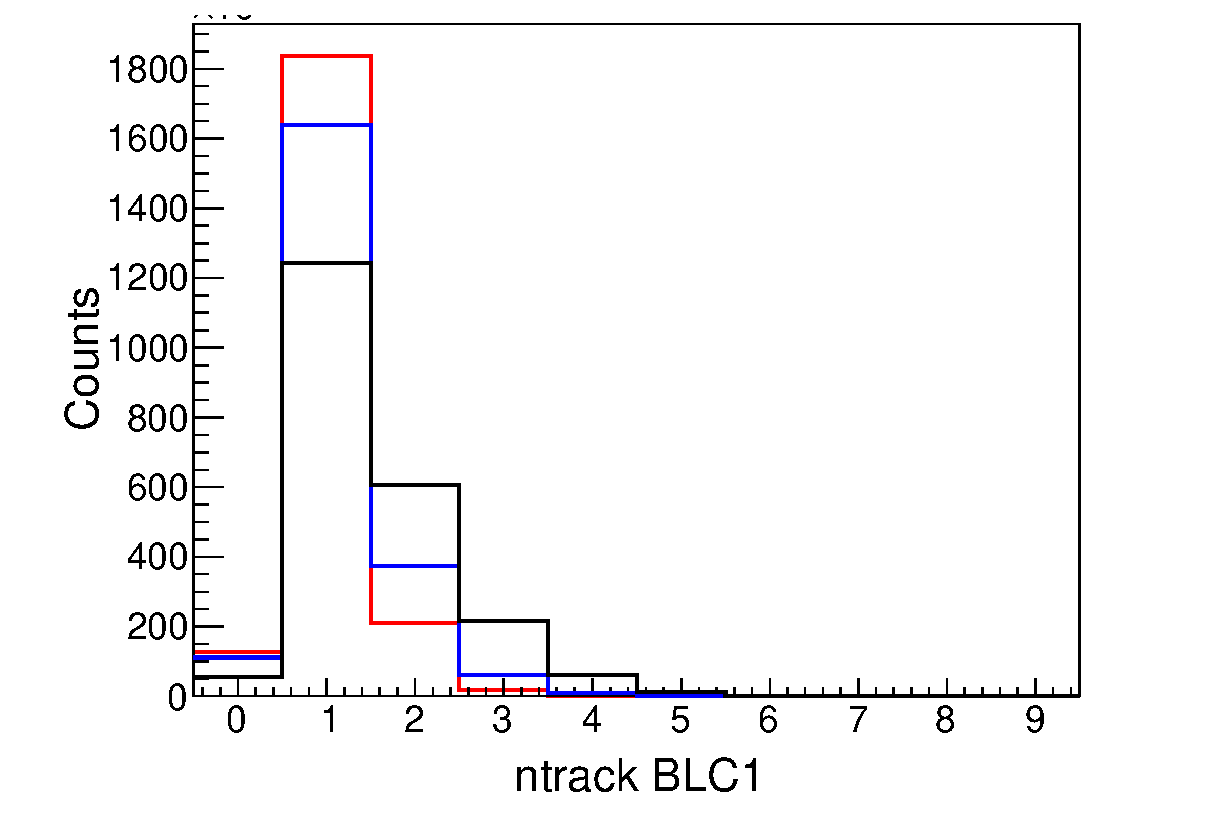
\includegraphics[width=4cm]{../pic/Run78/BL/nBLC1.eps}
    \end{minipage}
    \begin{minipage}{0.33\hsize}
      \includegraphics[width=4cm]{../pic/Run78/BL/BLC1_time.eps}
    \end{minipage}
    \begin{minipage}{0.33\hsize}
      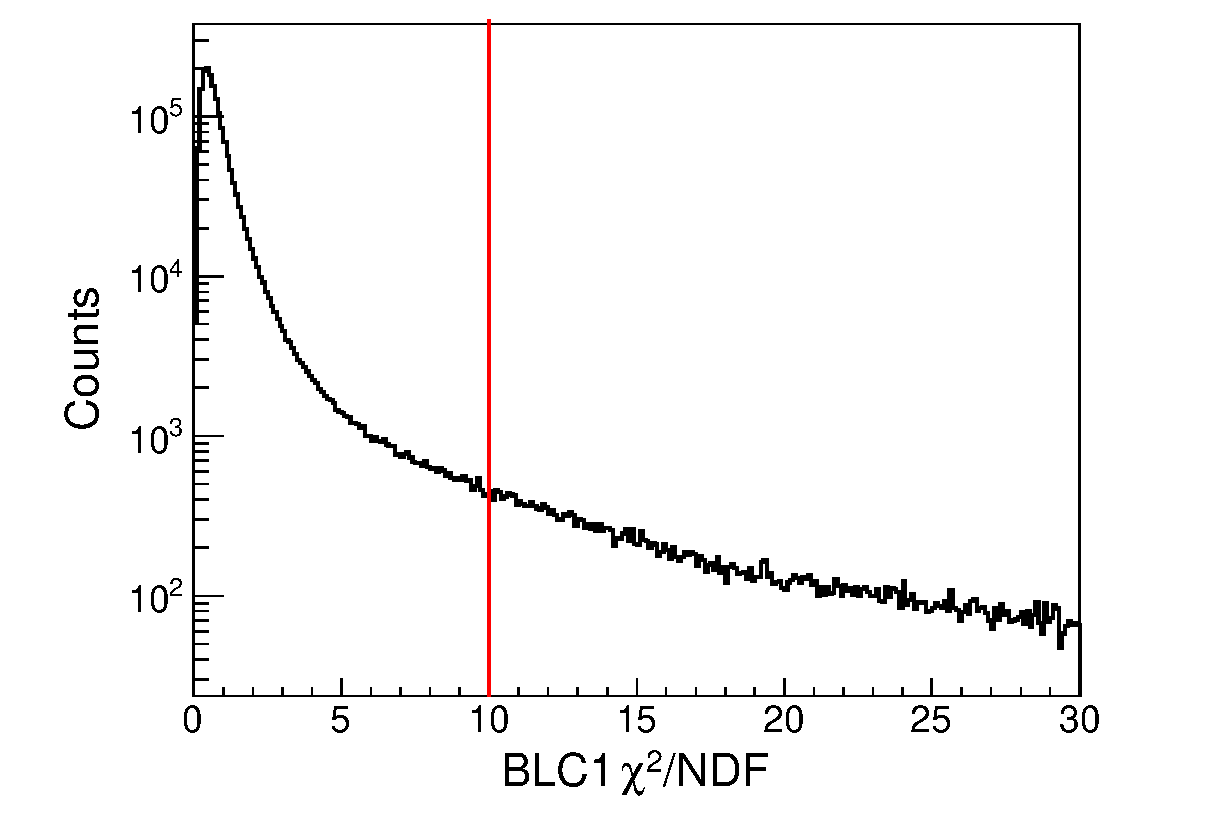
\includegraphics[width=4cm]{../pic/Run78/BL/BLC1_chi2.eps}
    \end{minipage}
  \end{tabular}
  
  \begin{tabular}{ccc}
    \begin{minipage}{0.33\hsize}
      \includegraphics[width=4cm]{../pic/Run78/BL/nBLC2.eps}
    \end{minipage}
    \begin{minipage}{0.33\hsize}
      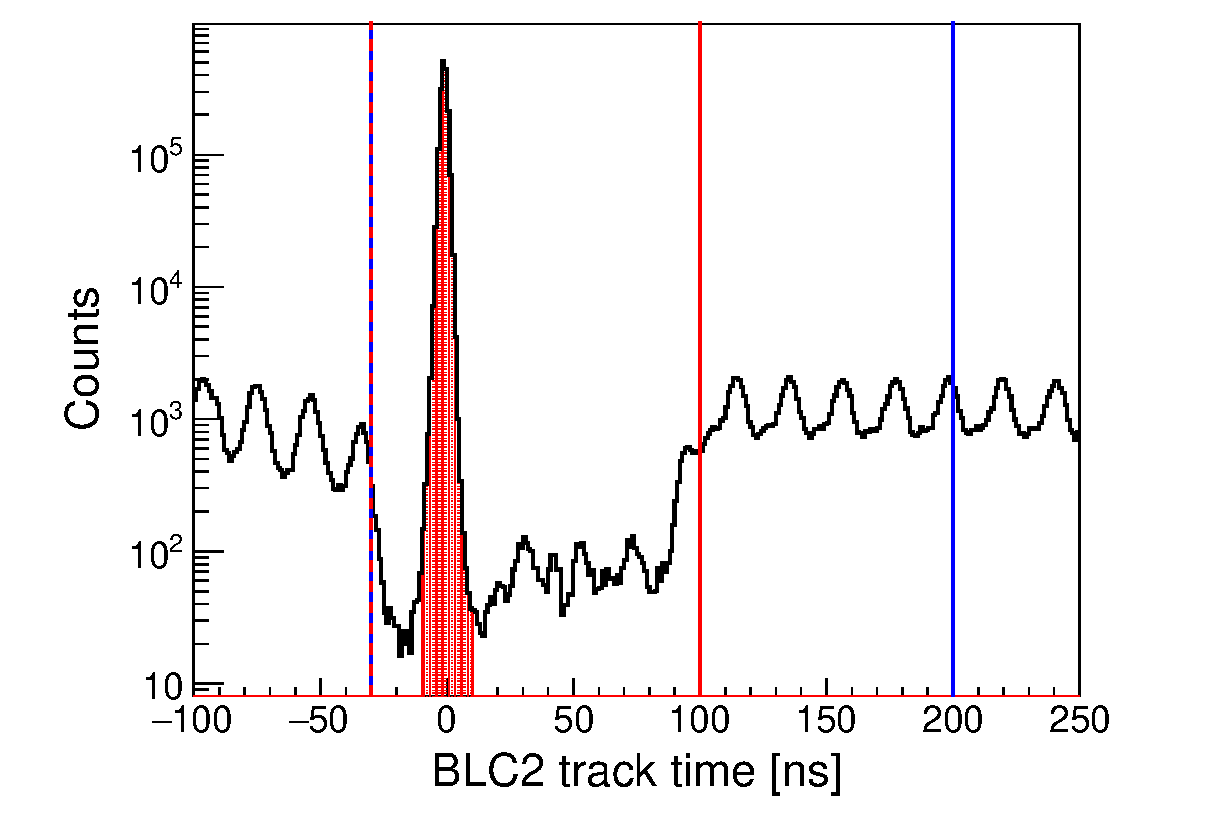
\includegraphics[width=4cm]{../pic/Run78/BL/BLC2_time.eps}
    \end{minipage}
    \begin{minipage}{0.33\hsize}
      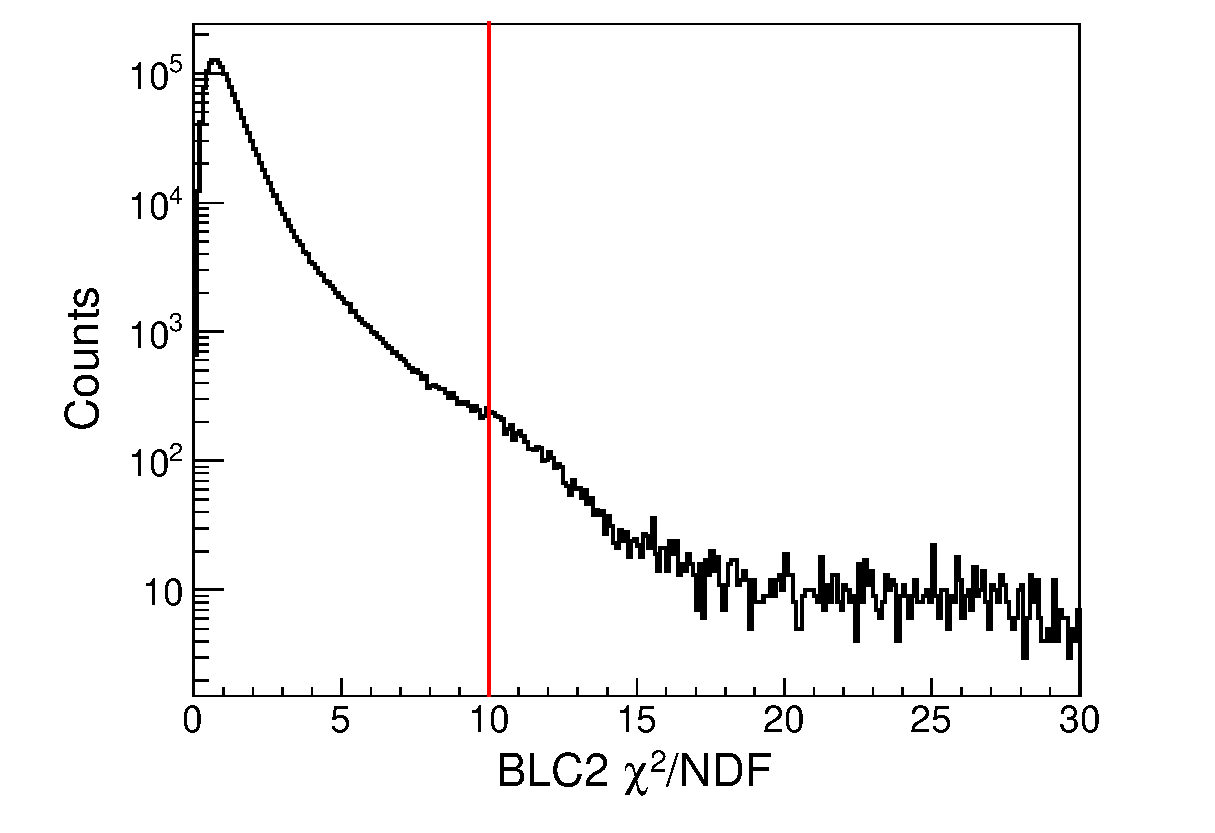
\includegraphics[width=4cm]{../pic/Run78/BL/BLC2_chi2.eps}
    \end{minipage}
  \end{tabular}
  
  \begin{tabular}{ccc}
    \begin{minipage}{0.33\hsize}
      \includegraphics[width=4cm]{../pic/Run78/BL/nBPC.eps}
    \end{minipage}
    \begin{minipage}{0.33\hsize}
      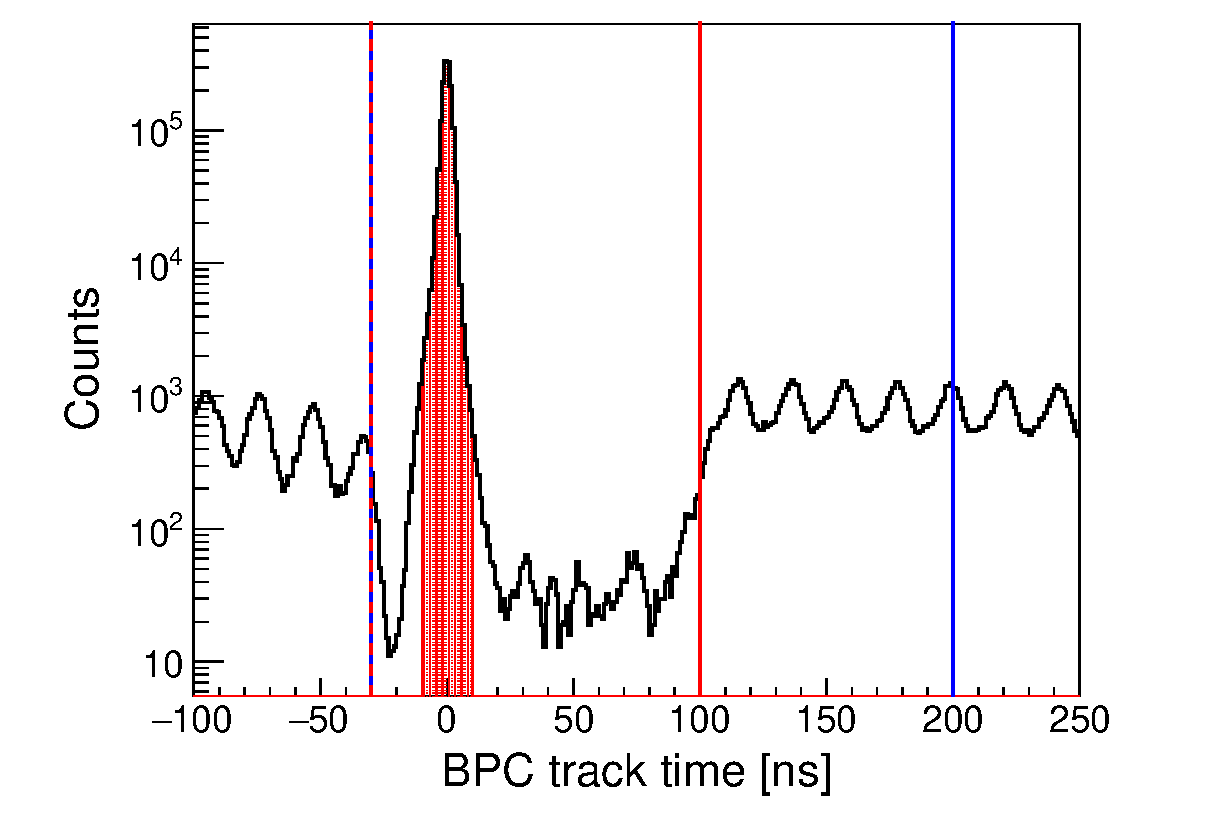
\includegraphics[width=4cm]{../pic/Run78/BL/BPC_time.eps}
    \end{minipage}
    \begin{minipage}{0.33\hsize}
      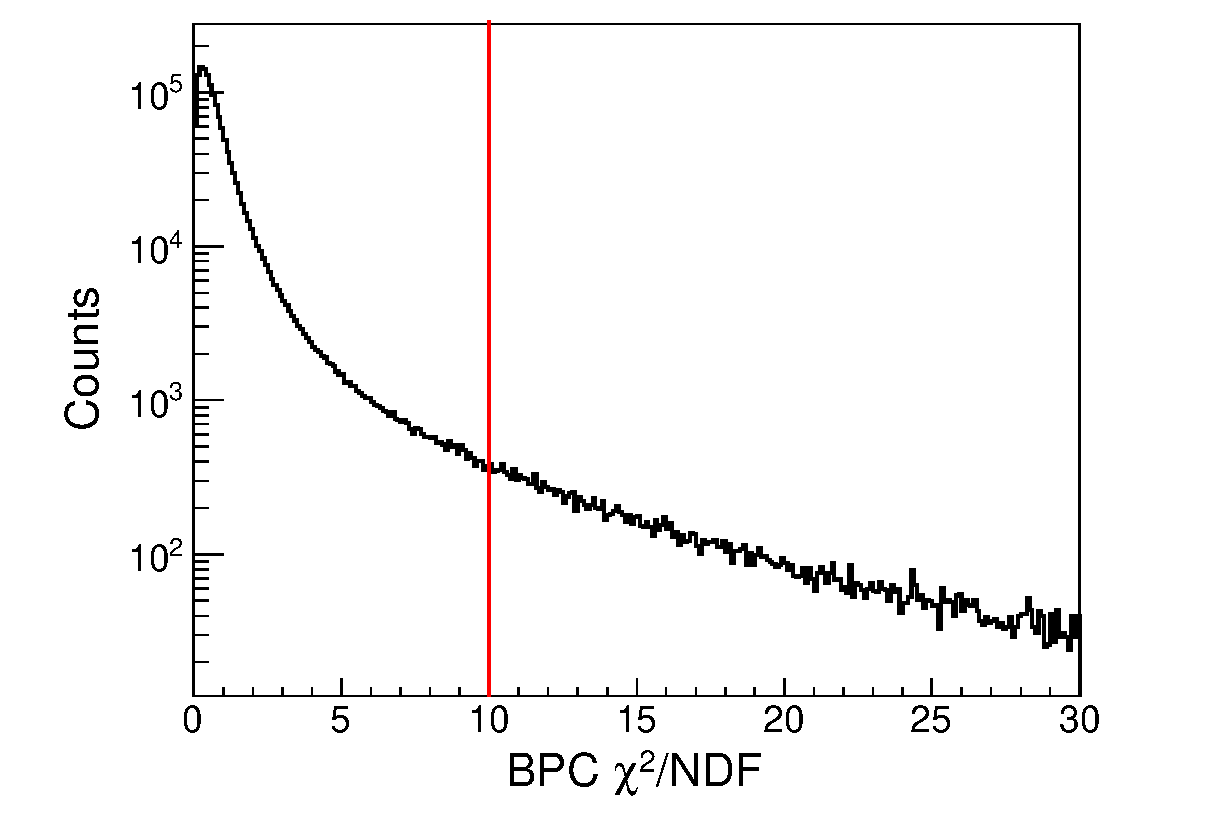
\includegraphics[width=4cm]{../pic/Run78/BL/BPC_chi2.eps}
    \end{minipage}
  \end{tabular}
  \caption{
    The left, the middle and the right figures show the number of tracks, track time and $\chi/NDF$, respectively.
    Color plots in the left figure indicate some time window.
    % Black, blue, red indicate all, $-30\sim200$[ns], $-30\sim100$[ns], respectively.
    The above, the middle and the down figures represent BLC1, BLC2 and BPC, respectively.
    The BPC was described after.
  }
  \label{fig:BLC_etc}
\end{figure}
BLC1 and BLC2 were installed upstream and downstream of the D5 magnet, respectively to measure beam momentum using the transfer matrix of the D5 magnet.
These are planer the type drift chamber whose drift length was calculated using the X-T map, which was the integration of drift time.
The track time of BLC was estimated from timing signals of pair plane due to constant drift length.
SX beam has RF-structure seems like the center figures of Fig\ref{fig:BLC_etc}, so we select synchronization about beam which indicates the red hatched region.
The left figures represent the number of tracks, in which black, blue, and red indicate time window of all, $-30\sim100$[ns], and $-30\sim200$[ns], respectively.
We select 1track events in red time window selection to keep statistics.
The right figures show $\chi^2/NDF$ distribution after 1track selection.
We accepted $\chi^2/NDF<10$ events as good track.

\begin{frame}{Beam momentum analysis by D5}
  \begin{tabular}{cc}
    \begin{minipage}{0.5\hsize}
      \begin{figure}
        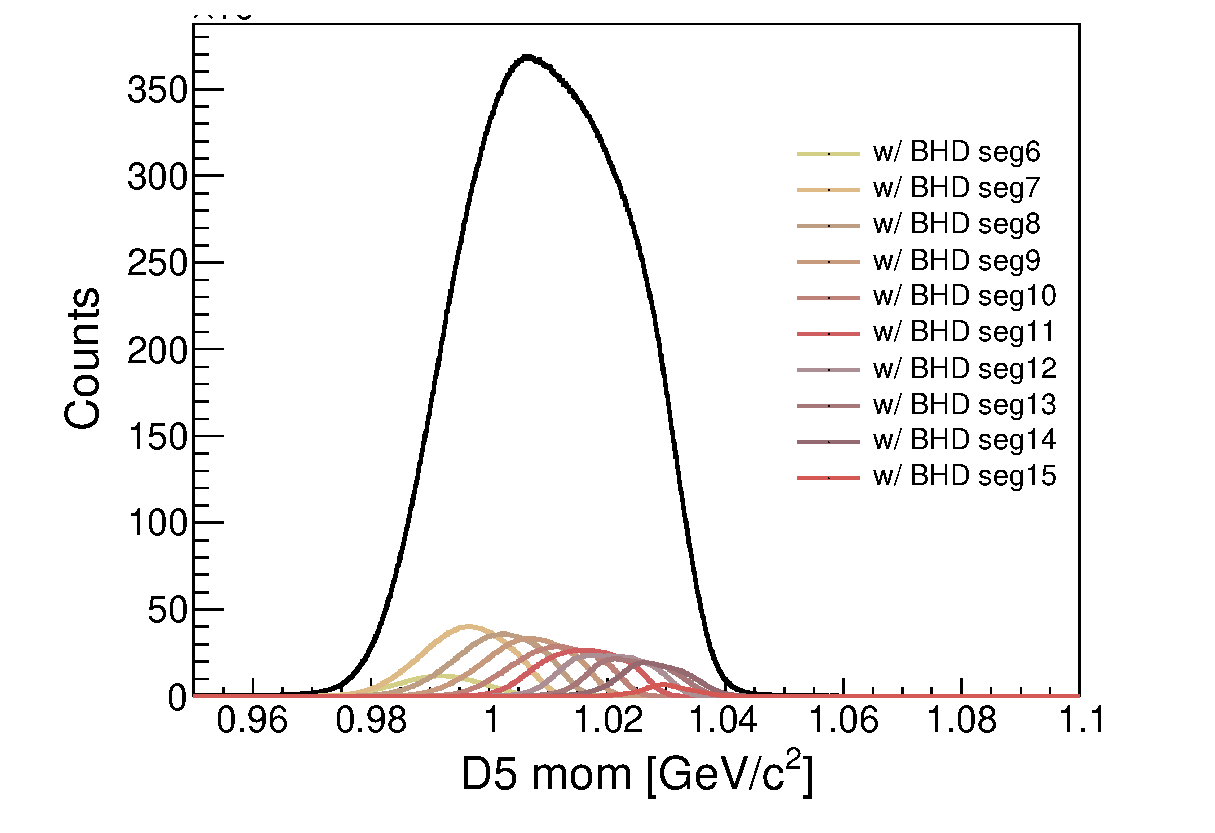
\includegraphics[width=5cm]{../pic/Run78/BL/D5_mom.eps}
      \end{figure}
    \end{minipage}

    \begin{minipage}{0.5\hsize}
      \begin{figure}
        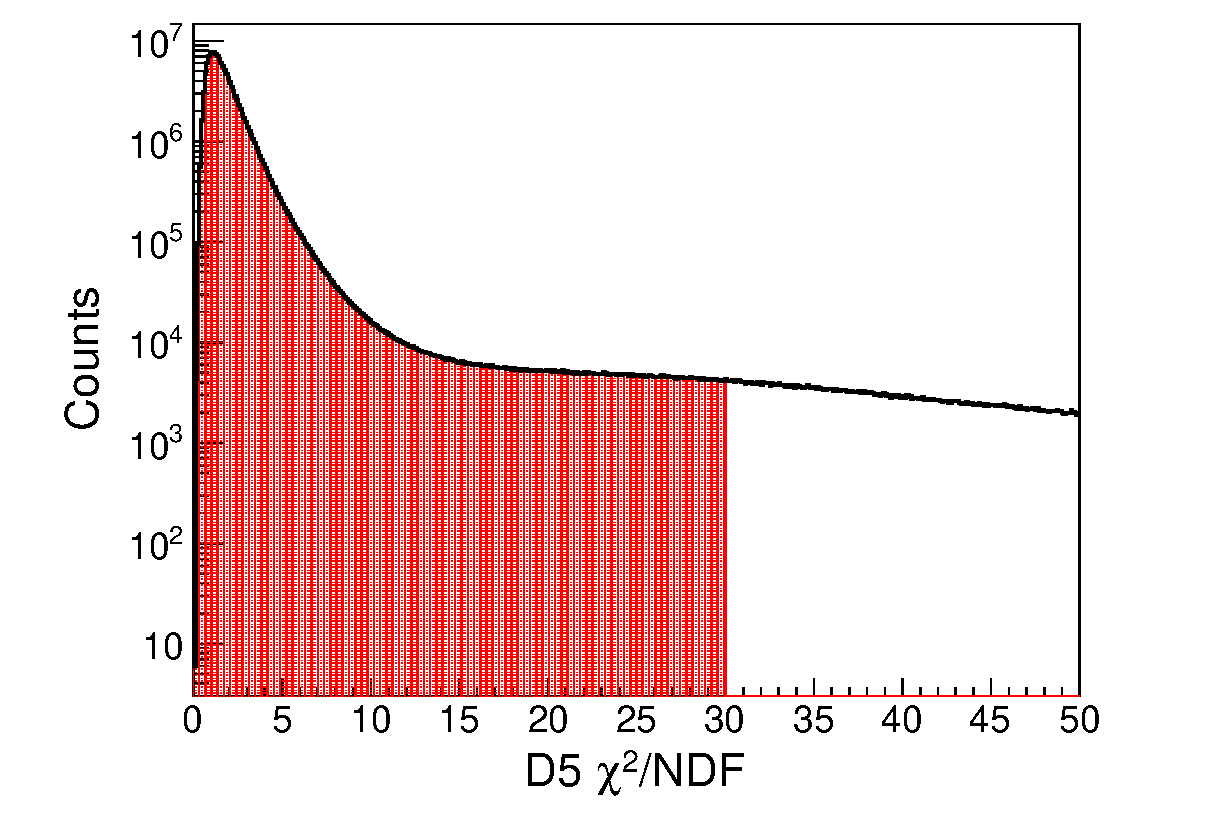
\includegraphics[width=5cm]{../pic/Run78/BL/D5_chi2.eps}
      \end{figure}
    \end{minipage}
  \end{tabular}


  \begin{tabular}{cc}
    \begin{minipage}{0.5\hsize}
      \begin{figure}
        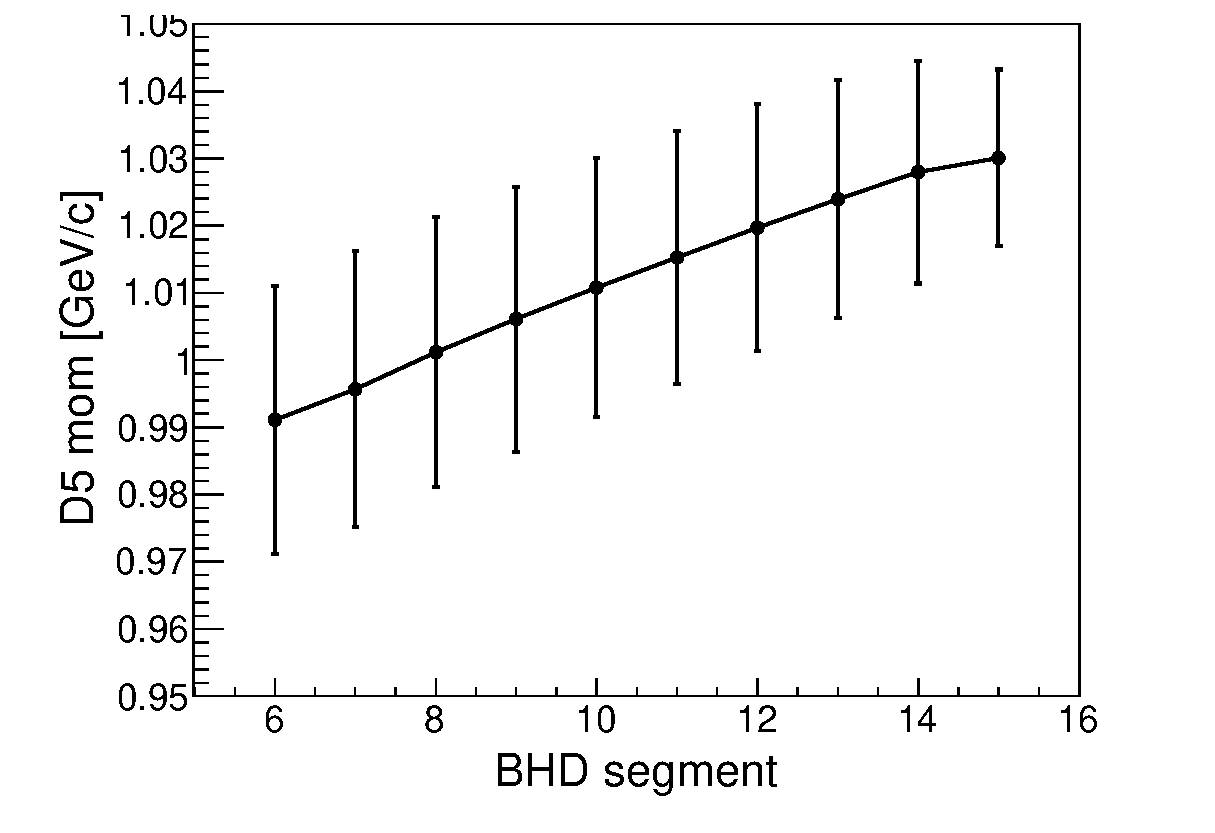
\includegraphics[width=5cm]{../pic/Run78/BL/D5_mom_BHDseg.eps}
      \end{figure}
    \end{minipage}

    \begin{minipage}{0.5\hsize}
      D5 momentum has a correlation about BHD segment.
    \end{minipage}
  \end{tabular}



\end{frame}

\subsection{BLC2-BPC matching}
\begin{figure}[htpb]
  \centering
  \begin{tabular}{cc}
    \begin{minipage}{0.5\hsize}
      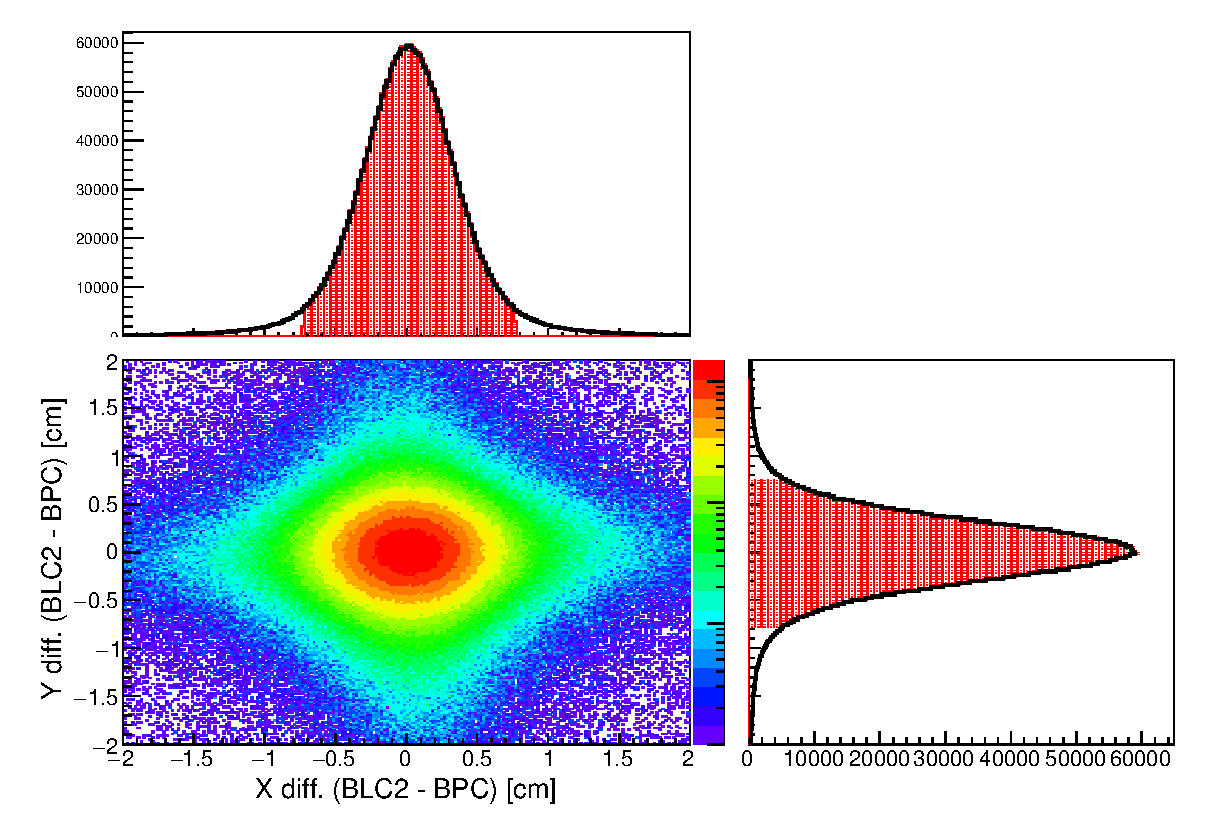
\includegraphics[width=6cm]{../pic/Run78/BL/BLC2BPC.eps}
    \end{minipage}
    \begin{minipage}{0.5\hsize}
      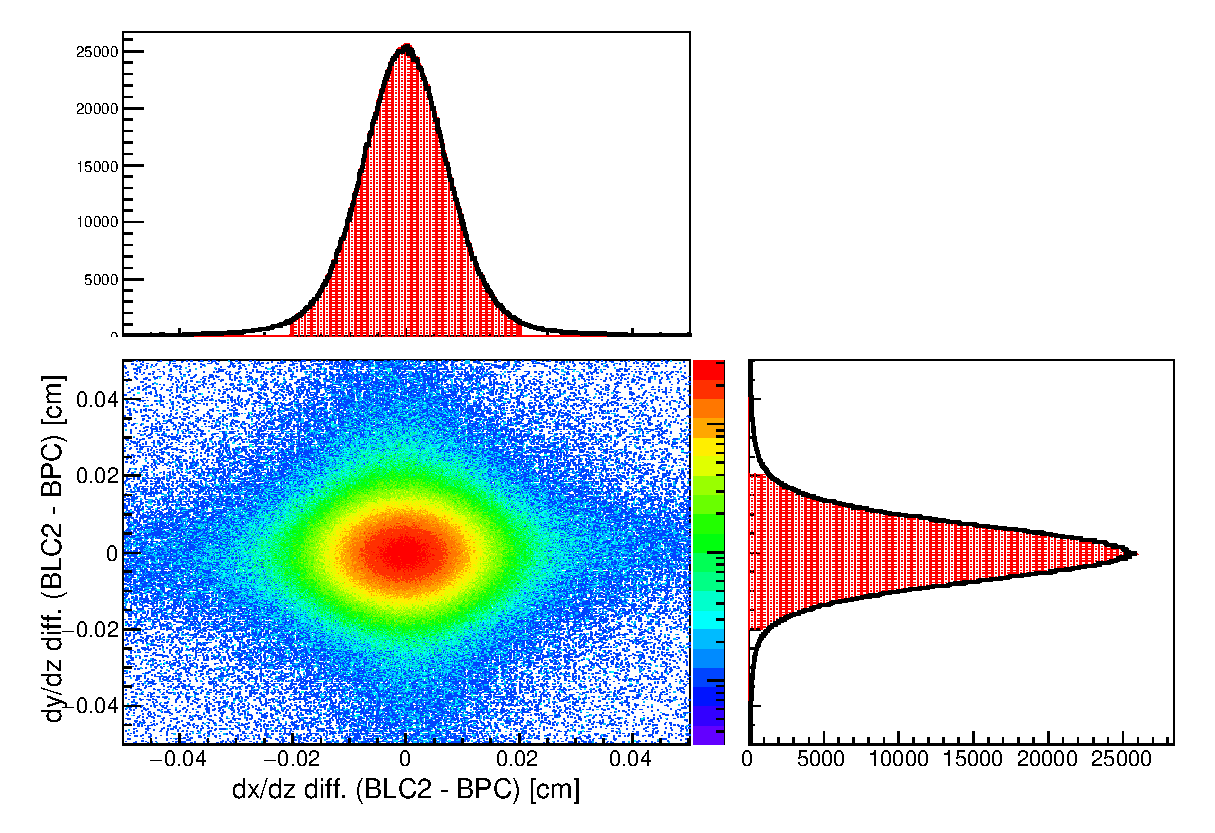
\includegraphics[width=6cm]{../pic/Run78/BL/BLC2BPC_dir.eps}
    \end{minipage}
  \end{tabular}
  \caption{
    These figures indicate the connection between the BLC2 and the BPC.
    The left figure shows about position matching at the center of these.
    The right figure shows direction matching.
    The red hatched region indicated an acceptable region.
  }
  \label{fig:BLC2BPC}
\end{figure}

\begin{figure}[htpb]
  \begin{tabular}{cc}
    \begin{minipage}{0.5\hsize}
      \includegraphics[width=6cm]{../pic/Run78/BL/profFF_Kf.eps}
    \end{minipage}
    \begin{minipage}{0.5\hsize}
      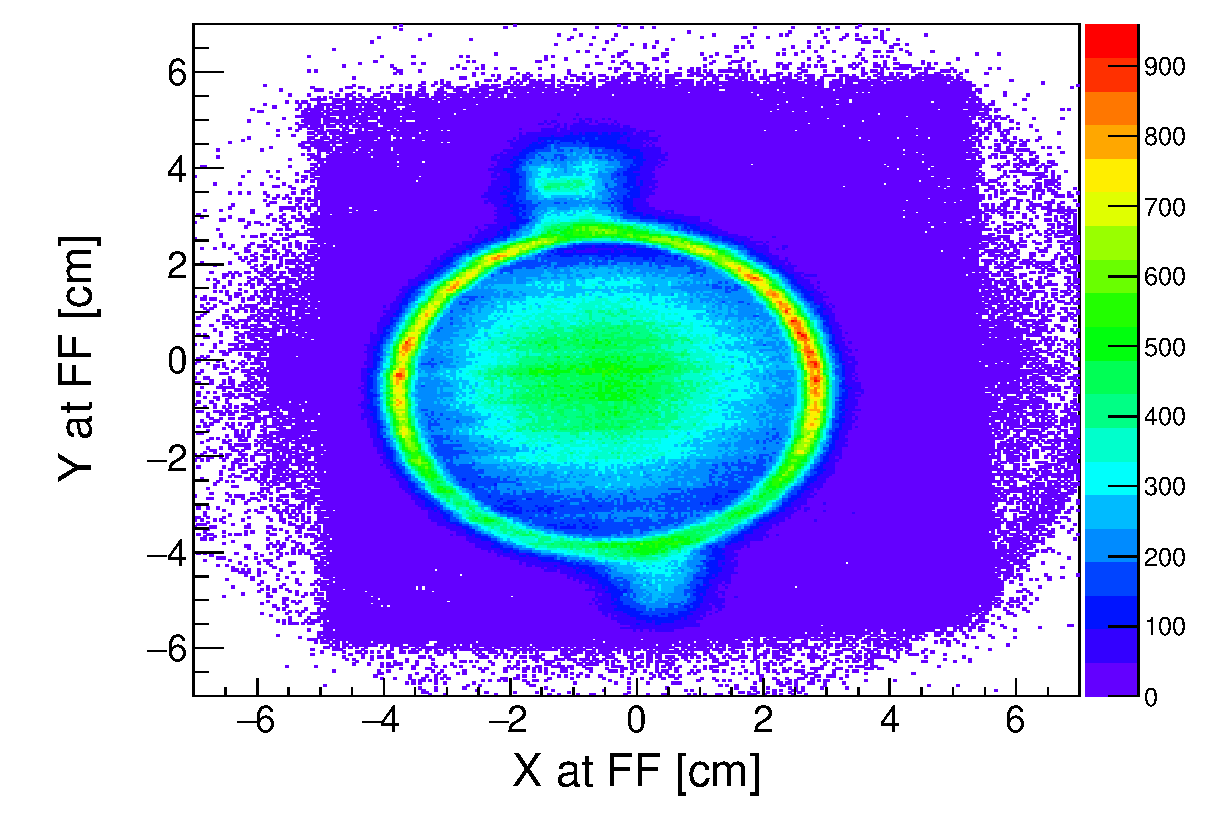
\includegraphics[width=6cm]{../pic/Run78/BL/profFF_KCDH2.eps}
    \end{minipage}
  \end{tabular}
  \caption{
    These figures shows beam profile at FF.
    The left figure shows about the unbiased kaon trigger.
    The right figure shows about CDH2 hit trigger.
  }
  \label{fig:profFF}
\end{figure}
The BPC is the same type drift chamber as BLC1/2, so the analysis of itself is the same as BLC1/2, which is shown in Fig\ref{fig:BLC_etc}.
There is no magnet between the BLC2 and the BPC, so trajectories reconstructed by them sshould be successfully connected within multiple scattering and resolution.
There are many materials between the BLC2 and the BPC, for example, the T0, the AC, BPD, and air, also direction ($dx/dz$ or $dy/dz$) resolution affects on extracted position resolution.
The $z$ length ratio of these is (BPC $z$)/(BLC2 $z$)=50.4mm/310mm$\sim$1/6, so extracted position resolution was almost decided by the BPC.
On the other hand, materials were placed at just down stream of the BLC2 for example the T0 and the AC.
These two effects were estimated almost the same, so we evaluated position matching at the center of the BLC2 and the BPC as Fig\ref{fig:BLC2BPC}.
We also require direction matching the right figure of Fig\ref{fig:BLC2BPC}.
The BPC also defines The beam profile at the experimental target position as shown in Fig\ref{fig:profFF}.
The profile required reaction at the trigger level was clearly seen target cell.
The red circle indicates an acceptable region as an effective kaon beam. %% todo Fiducialの赤枠

\begin{frame}{Profile at Final Forcus}
  \begin{tabular}{cc}
    \begin{minipage}{0.5\hsize}
      \begin{figure}
        Unbaised Kaon Trig.\\
        \includegraphics[width=6cm]{../pic/Run78/BL/profFF_Kf.eps}
      \end{figure}
    \end{minipage}

    \begin{minipage}{0.5\hsize}
      \begin{figure}
        CDH2 Trig.\\
        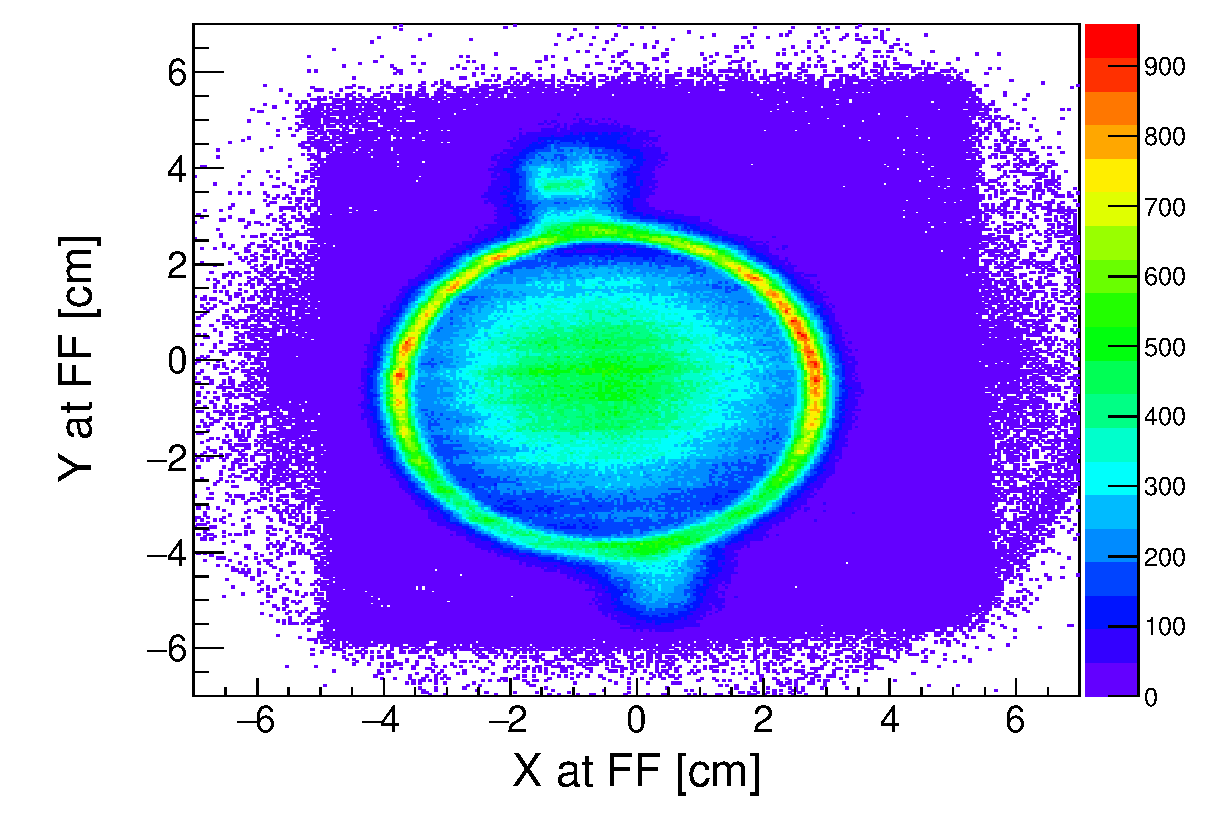
\includegraphics[width=6cm]{../pic/Run78/BL/profFF_KCDH2.eps}
      \end{figure}
    \end{minipage}
  \end{tabular}
\end{frame}



\begin{frame}
  \label{page:CDS}
  { \Huge CDS Analysis }
\end{frame}
\begin{frame}{CDC fine turning}
  \begin{tabular}{cc}
    \begin{minipage}{0.5\hsize}
      \begin{figure}
        Before\\
        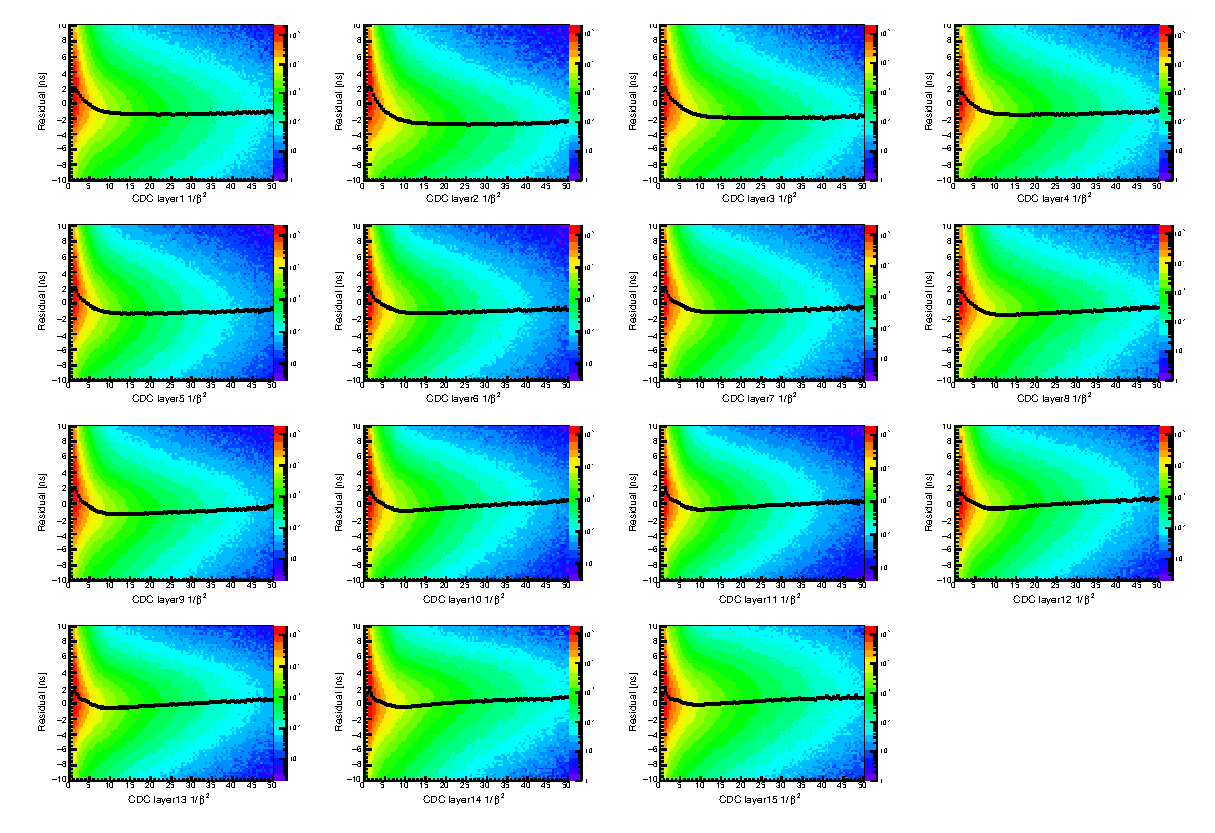
\includegraphics[width=5cm]{../pic/Run78/CDS/CDC_ob2_res_before.eps}
      \end{figure}
    \end{minipage}

    \begin{minipage}{0.5\hsize}
      \begin{figure}
        After\\
        \includegraphics[width=5cm]{../pic/Run78/CDS/CDC_ob2_res.eps}
      \end{figure}
    \end{minipage}
  \end{tabular}
  \centering
  $\beta$ and residual has correlation, which was calibrated wire-by-wire.
\end{frame}

\begin{frame}{Vertex image by CDS and BPC}
  \begin{figure}
    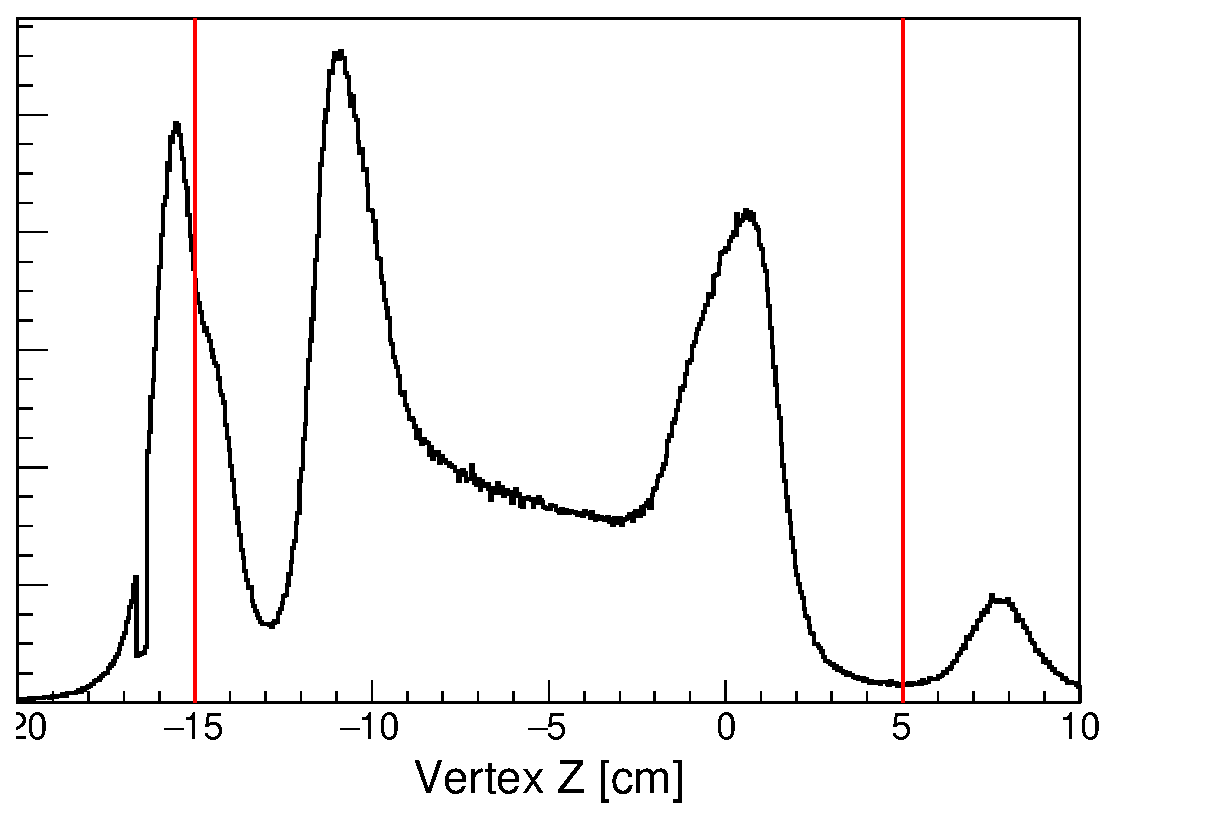
\includegraphics[width=8cm]{../pic/Run78/CDS/vertex.eps}
  \end{figure}
\end{frame}

\begin{frame}{Vertex image by CDS and BPC (Vertex cut)}
  \begin{figure}
    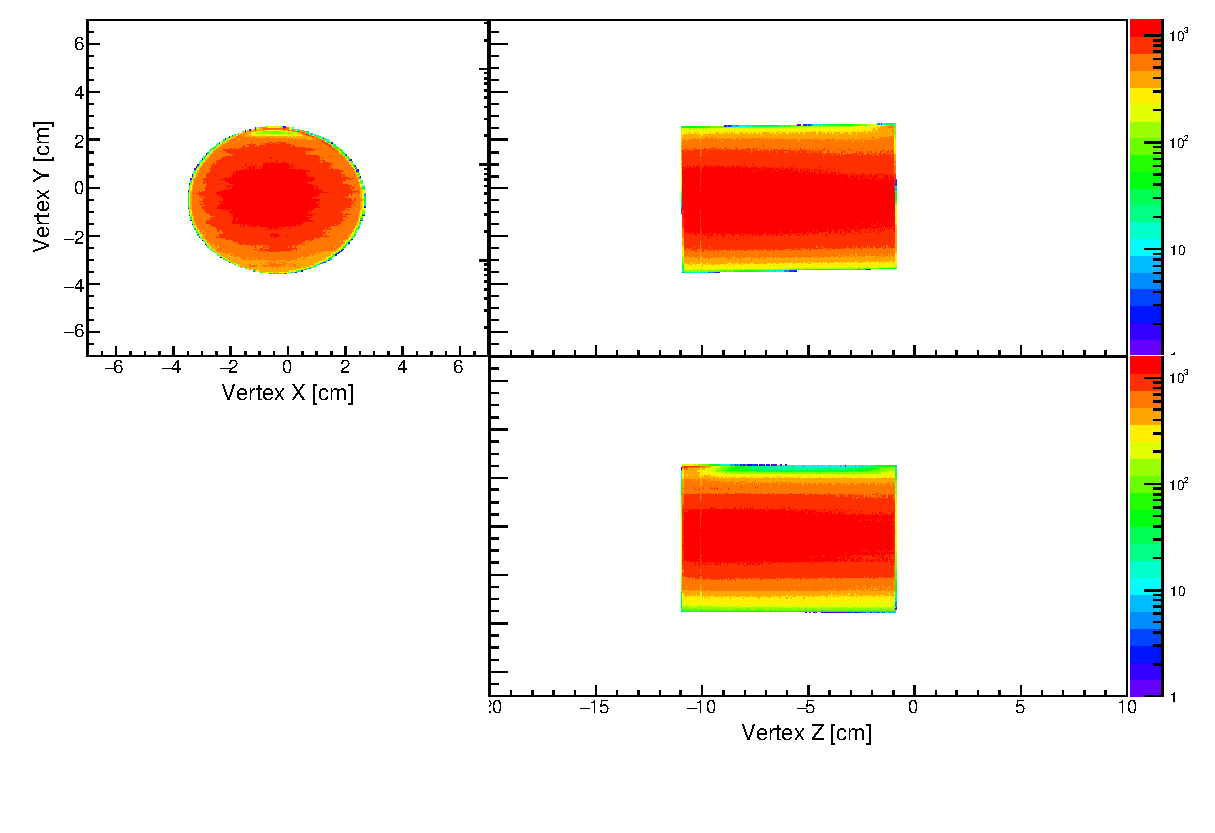
\includegraphics[width=8cm]{../pic/Run78/CDS/vertex_f.eps}
  \end{figure}
\end{frame}

\begin{frame}{Vertex resolution}
  \begin{tabular}{cc}
    \begin{minipage}{0.5\hsize}
      \begin{figure}
        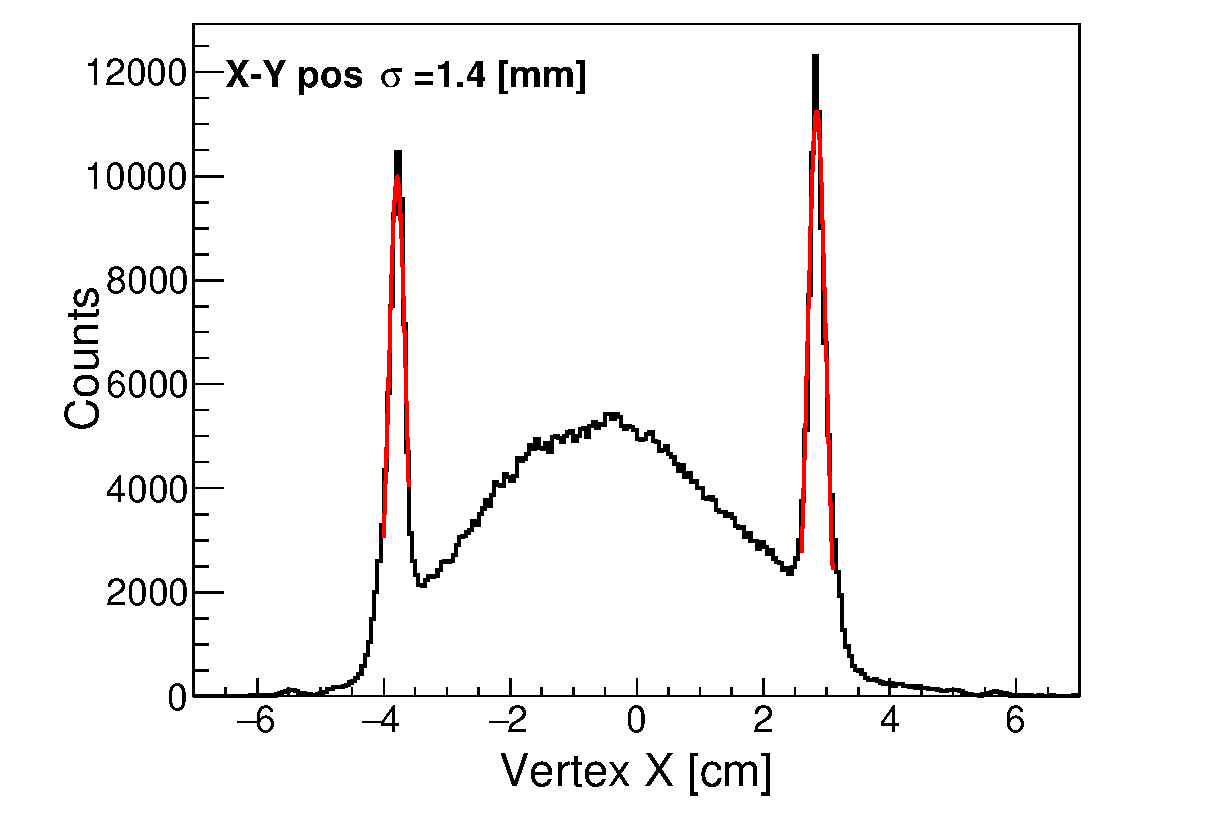
\includegraphics[width=5cm]{../pic/Run78/CDS/vertex_x.eps}
      \end{figure}
      \centering
      Y range was selected \\ $-5.5\sim-5$ [mm]
    \end{minipage}

    \begin{minipage}{0.5\hsize}
      \begin{figure}
        \includegraphics[width=5cm]{../pic/Run78/CDS/vertex_z.eps}
      \end{figure}
      \centering
      $Z =0$ was selected [mm]\\
      resolution was evaluated by DEF.
    \end{minipage}
  \end{tabular}
\end{frame}

\begin{frame}{CDS mass$^2$ vs momentum}
  \begin{figure}
    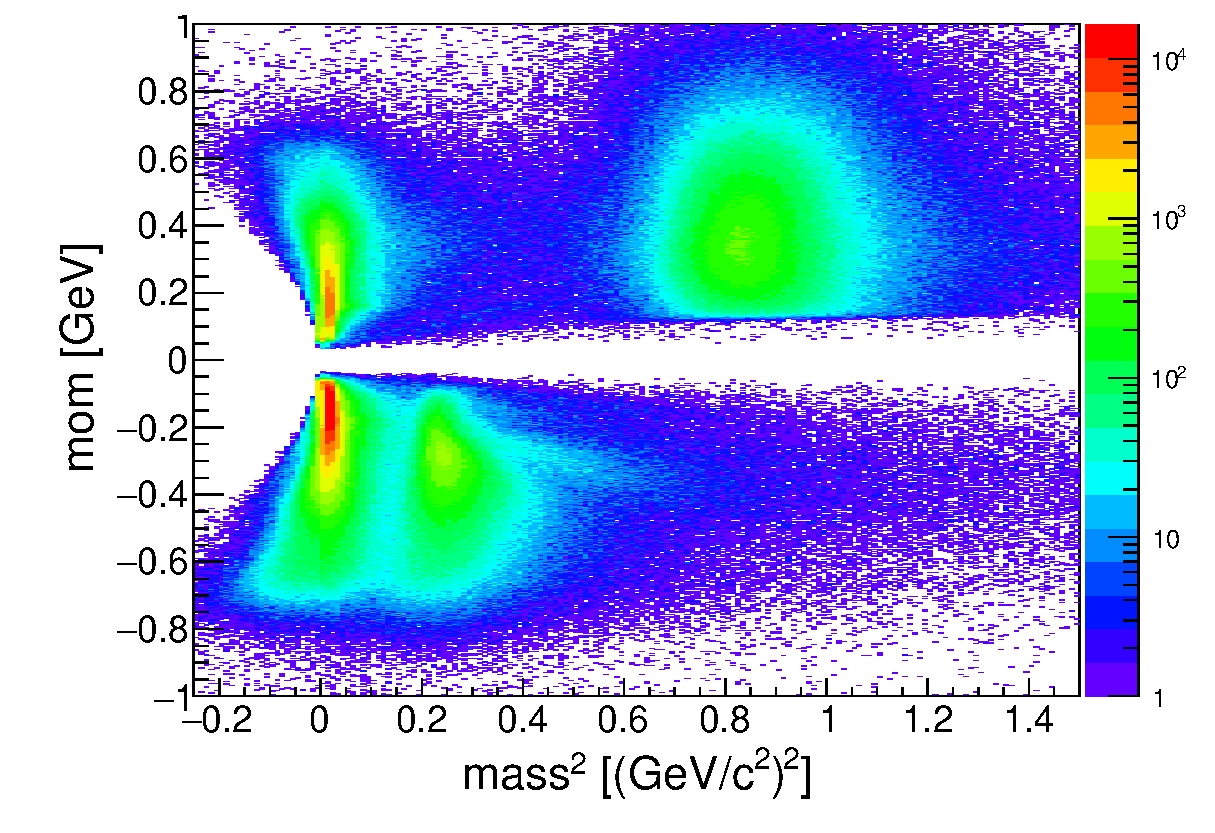
\includegraphics[width=8cm]{../pic/Run78/CDS/pid.eps}
  \end{figure}
\end{frame}

\begin{frame}{Invaraint mass by CDS}
  \begin{tabular}{cc}
    \begin{minipage}{0.5\hsize}
      \begin{figure}
        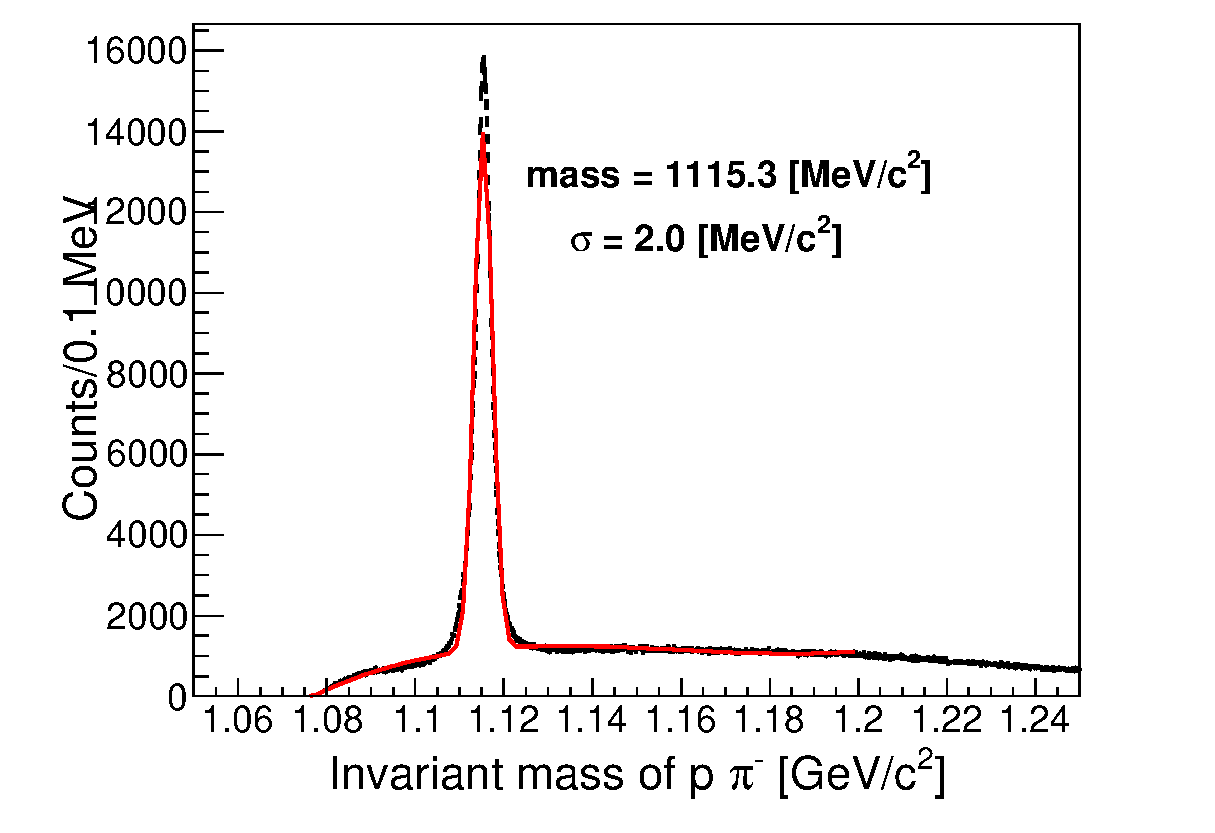
\includegraphics[width=5cm]{../pic/Run78/CDS/IM_ppim.eps}
      \end{figure}
    \end{minipage}

    \begin{minipage}{0.5\hsize}
      \begin{figure}
        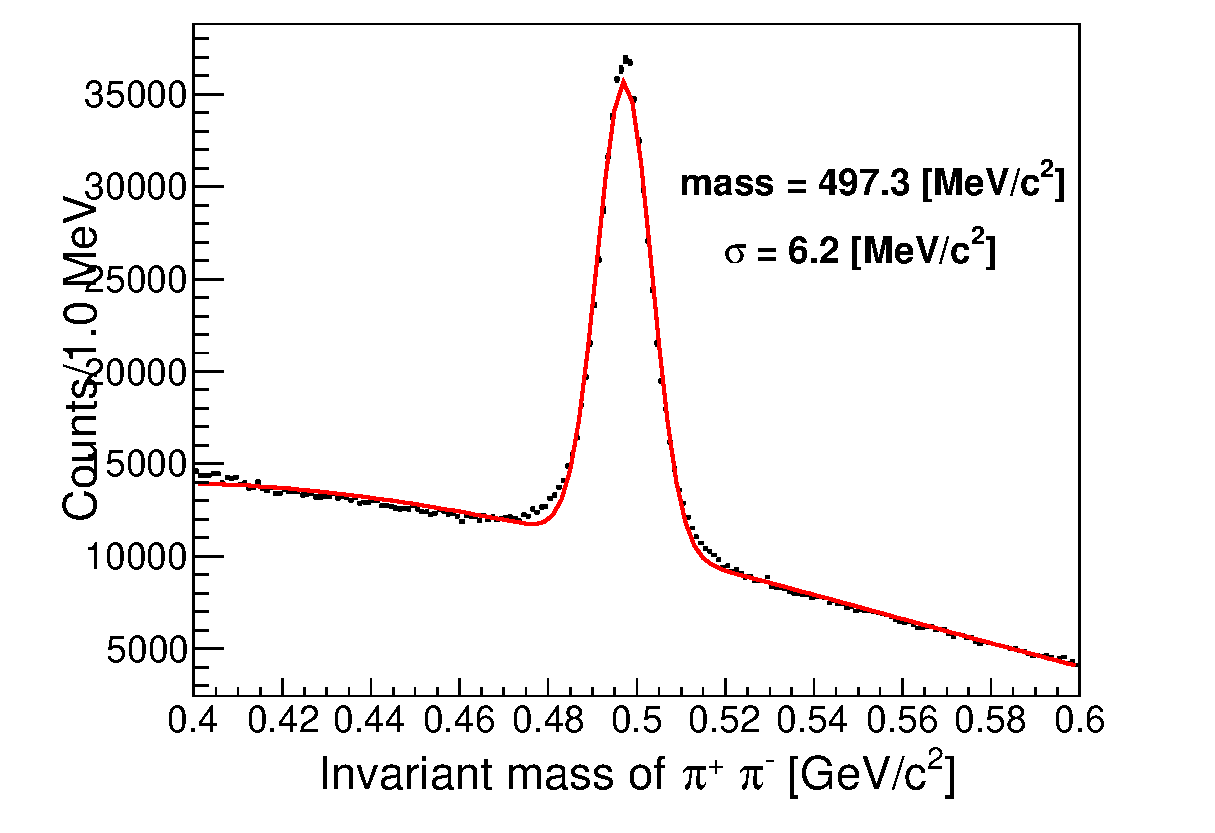
\includegraphics[width=5cm]{../pic/Run78/CDS/IM_pipi.eps}
      \end{figure}
    \end{minipage}
  \end{tabular}
\end{frame}




\begin{frame}
  \label{page:NC}
  { \Huge NC Analysis }
\end{frame}
\subsection{Neutron Counter - NC}
The neutron counter (NC) are located 14.7 m upstream of the target.
Because the NC are located at the most upstream and the purpose is to detecting neutral particles, the NC requires a large amount of material.
Therefore, the NC is a segmented scintillation detector with 7 layers, each layer consisting of 16 counters.
One scintillation detector is 20cm (width) $\times$ 150cm (height) $\times$ 5cm (thickness) in size.
So one layer covers 320cm (width) $\times$ 150cm (height), which is corresponds 6.2 degrees in horizontal and 2.9 degrees in vertical in this experiment setup.
The first three layers of the scintillator are made of Saint-Gobain BC408 and the other four layers are made of Saint-Gobain BC412.
The scintillation light is carried by lucite light guides on both sides and read out by the 2-inch PMT (Hamamatsu H6410).
Each layer is installed with a gap of 2 cm, so the whole NC has a thickness of 47 cm.
Differences between the upstream and downstream solid angles are evaluated as systematic errors.


\begin{frame}{$d(K^-, n)"\pi^{\pm}\Sigma^{\mp}"$ event selection}
  \begin{tabular}{cc}
    \begin{minipage}{0.5\hsize}
      { \scriptsize
        $d(K^-, n \pi^+ \pi^-)"n"$ was selected by 2$\sigma$.\\
        $K^- d \rightarrow K^0 n n $ was selected by 3$\sigma$.\\
        $K^- d \rightarrow \Sigma^{\pm}\pi^{\mp} n_{miss}$ was rejected by 3$\sigma$.
      }
      \begin{figure}
        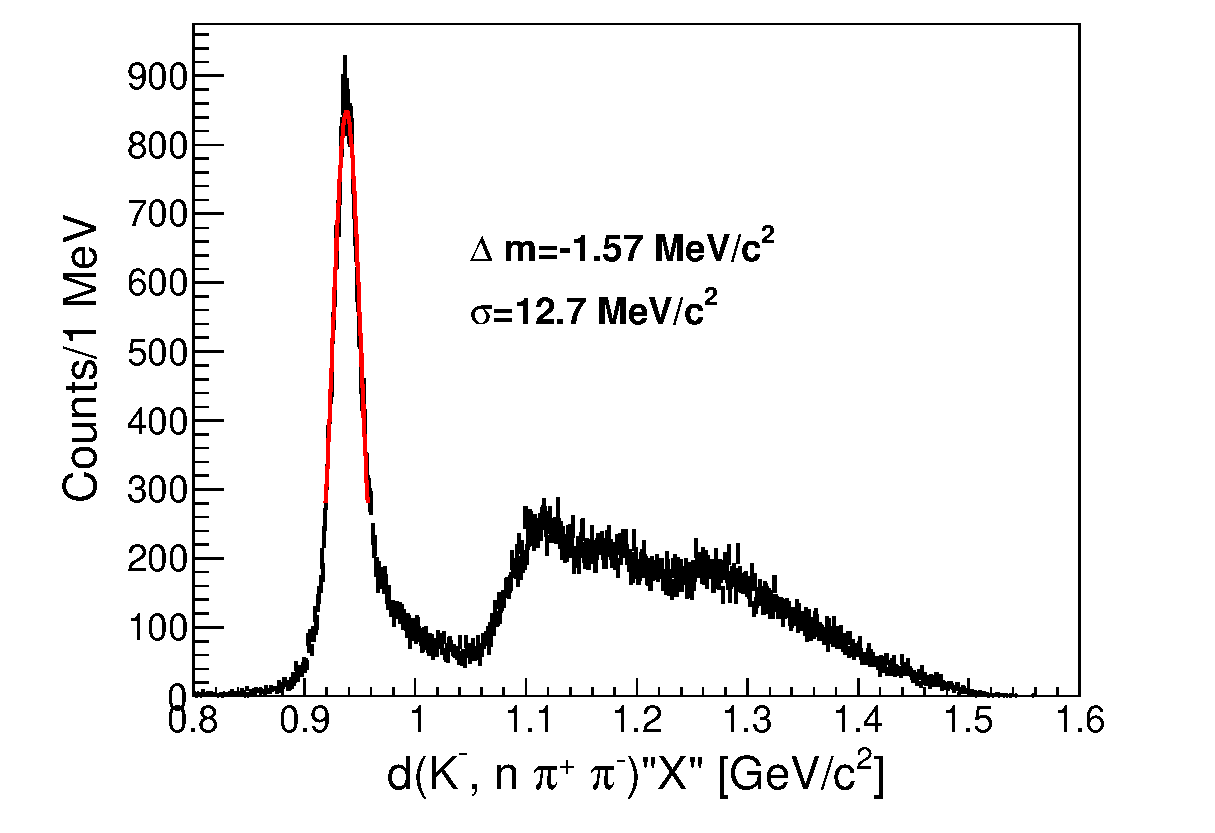
\includegraphics[width=5cm]{../pic/Run78/KN_ana_NC170_2sigma/KNpipi_MM_woFit.eps}
      \end{figure}
    \end{minipage}

    \begin{minipage}{0.5\hsize}
      \begin{figure}
        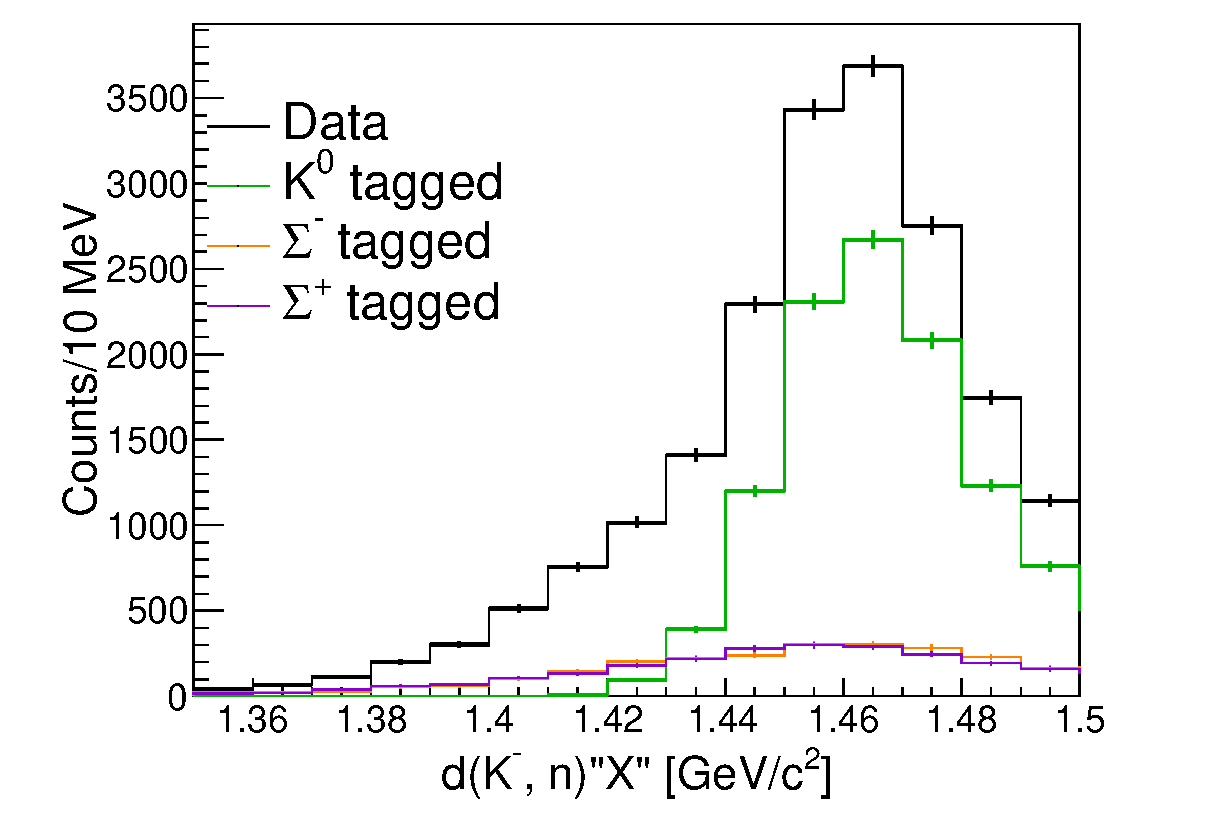
\includegraphics[width=6cm]{../pic/Run78/KN_ana_NC170_2sigma/KN_MM_all.eps}
      \end{figure}
    \end{minipage}
  \end{tabular}

  \begin{tabular}{cc}
    \begin{minipage}{0.33\hsize}
      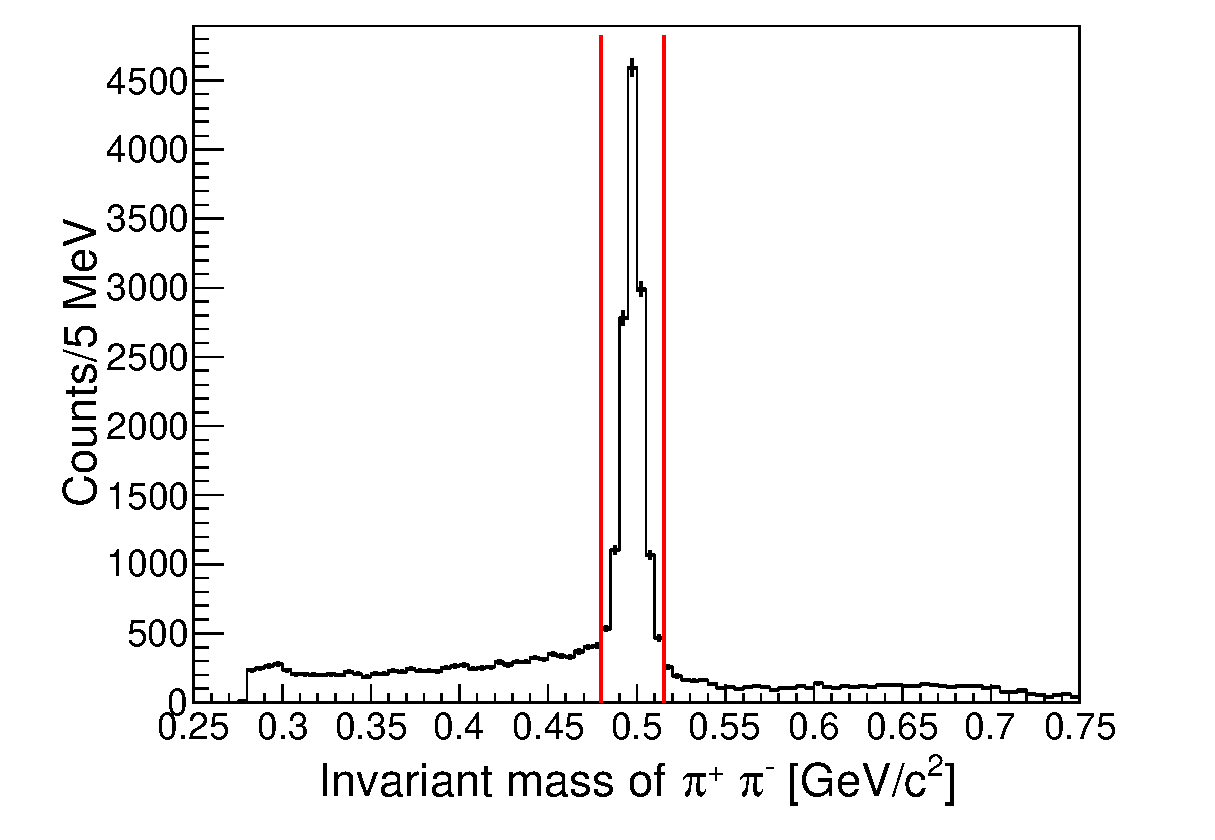
\includegraphics[width=3cm]{../pic/Run78/KN_ana_NC170_2sigma/IM_pipi_woFit.eps}
    \end{minipage}

    \begin{minipage}{0.33\hsize}
      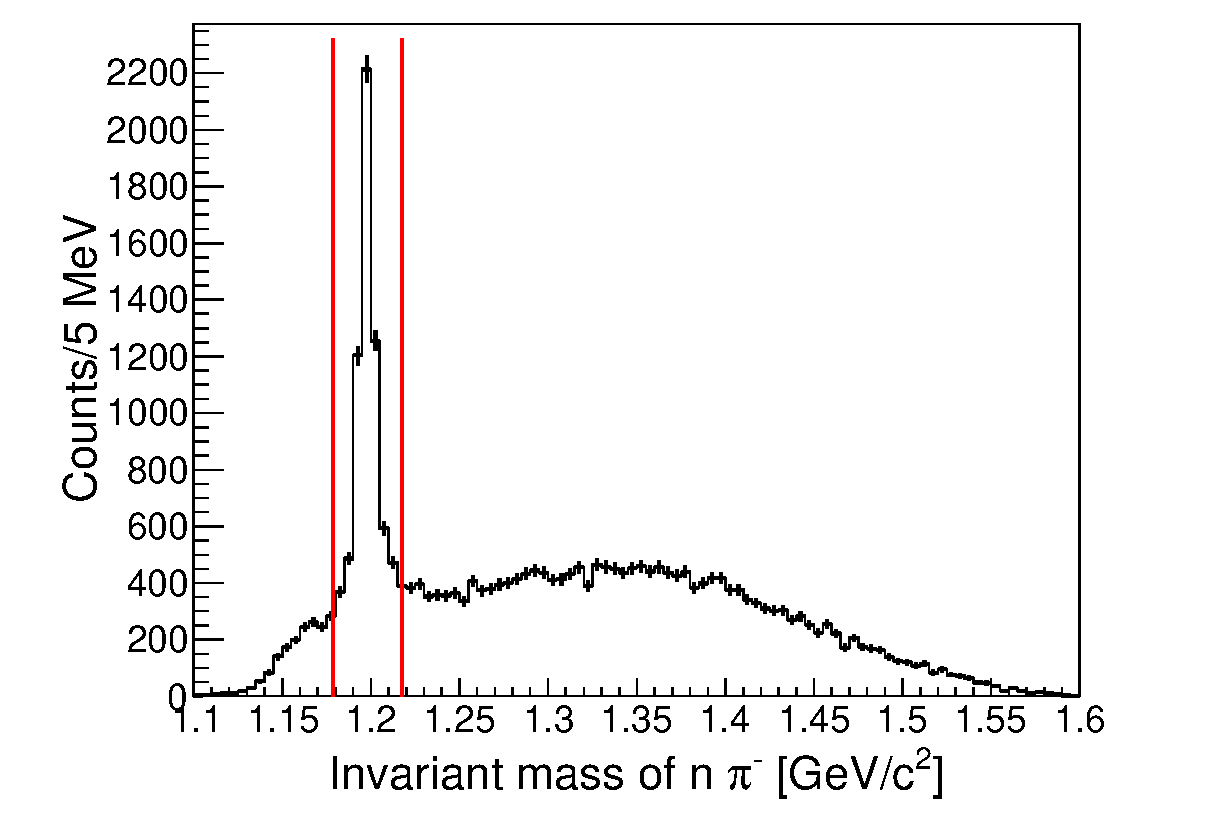
\includegraphics[width=3cm]{../pic/Run78/KN_ana_NC170_2sigma/IM_npim_woFit.eps}
    \end{minipage}

    \begin{minipage}{0.33\hsize}
      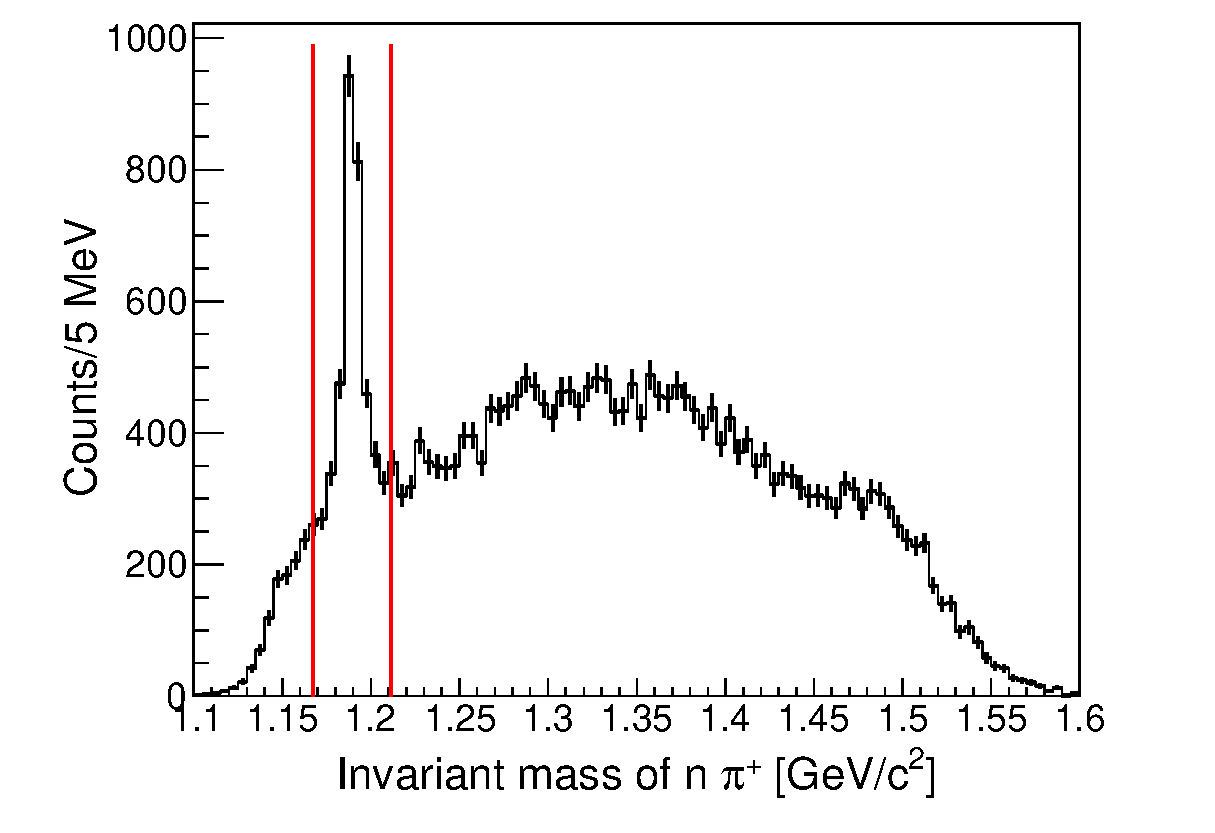
\includegraphics[width=3cm]{../pic/Run78/KN_ana_NC170_2sigma/IM_npip_woFit.eps}
    \end{minipage}
  \end{tabular}
\end{frame}


\begin{frame}{Reaction Identification}
  We expect these three reactions.
  \begin{itemize}
  \item $K^- d\rightarrow \pi^{\pm}"\Sigma^{\mp}" n_{forward}$ (Signal)
  \item $K^- d\rightarrow K^{0} n n$ (Quasi-elastic)
  \item $K^- d\rightarrow "n" \pi^{\pm} \Sigma^{\mp}_{forward}$ $\Sigma^{\mp}_{forward}\rightarrow n_{forward} \pi^{\mp}$
  \end{itemize}

  Identification method procedure.
  \begin{itemize}
  \item Three invariamt mass fitting of $\pi^+ \pi^-$, $n \pi^{\pm}$.\\
    $\rightarrow$ In this fitting, $K^- d\rightarrow \pi^{\pm}"\Sigma^{\mp}" n_{forward}$ was fixed.
    
  \item Missing mass of $d(K^-, n \pi^{\pm})"\Sigma^{\mp}"$ fitting.\\
    $\rightarrow$ In this fitting, $K^- d\rightarrow K^{0} n n$, $K^- d\rightarrow "n" \pi^{\pm} \Sigma^{\mp}_{forward}$ were fixed. \\
    $\rightarrow$ This fitting was performed bin-by-bin of $d(K^-, n)"X"$.\\
  \item These fitting was performed iterationary.
  \end{itemize}

  Fitting method was adopted below method.\\
  { \tiny
    \href{https://www.sciencedirect.com/science/article/pii/001046559390005W}{R. Barlow and C. Beeston, Comp. Phys. Comm. 77 (1993) 219-228 \\ \vspace{-3mm}
      "Fitting using finite Monte Carlo samples"}
  }
  
  { \tiny
    \href{https://www.sciencedirect.com/science/article/pii/S0010465508003652}{A.Nappi, Comp Phys. Comm. 180 (2009) 269-275 \\ \vspace{-3mm}
      "A pitfall in the use of extended likelihood for fitting fractions of pure samples in a mixed sample"}
  }
\end{frame}


\begin{frame}{$d(K^-, n \pi^+ \pi^-)"X"$ data and MC (NC $\sigma=150ps$)}
  \begin{itemize}
  \item $K^- d\rightarrow (\pi^{\pm}\Sigma^{\mp})_{backwoard} n_{forward}$ (Signal)
  \item $K^- d\rightarrow K^{0} n n$ (Quasi-elastic)
  \item $K^- d\rightarrow n \pi^{\pm} \Sigma^{\mp}_{forward}$ 

  \end{itemize}
  \begin{tabular}{cc}
    \begin{minipage}{0.6\hsize}
      \begin{figure}
        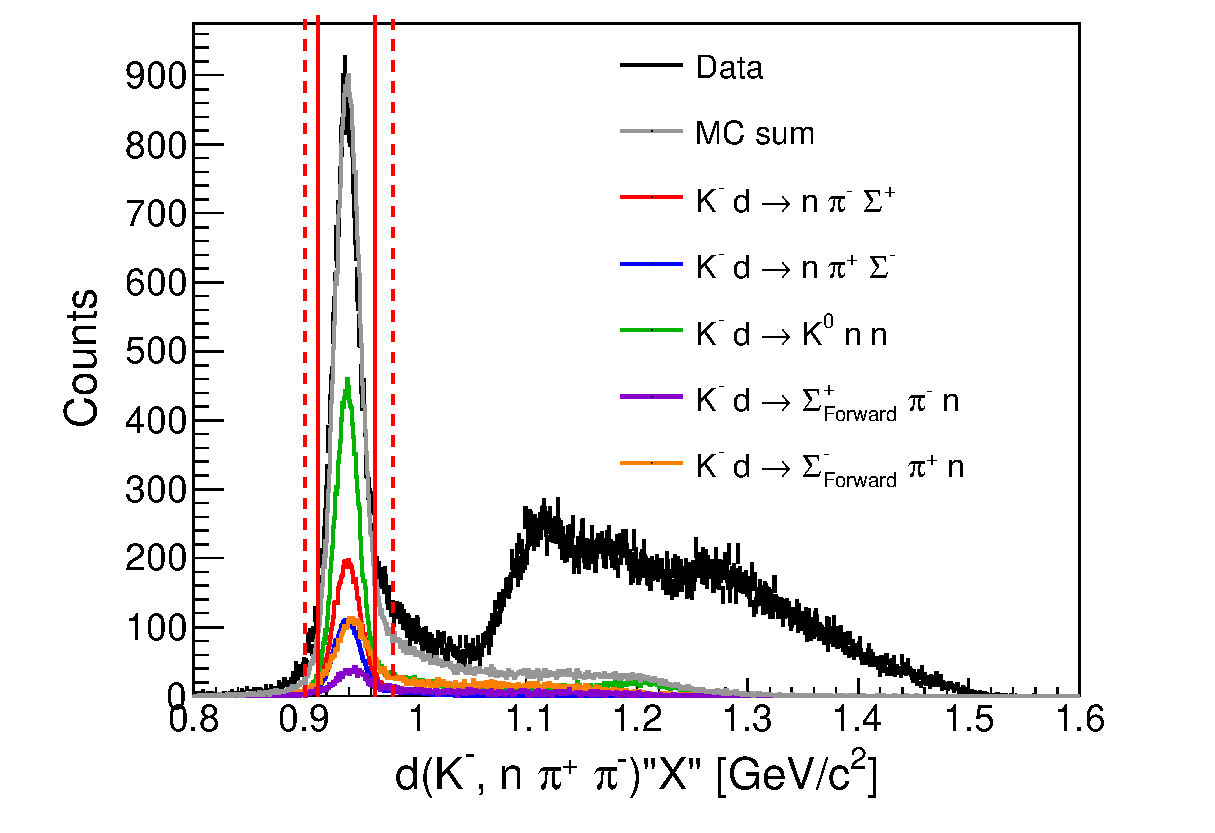
\includegraphics[width=6cm]{../pic/Run78/KN_ana_3sigma/fitKNpipi_MM.eps}
      \end{figure}
    \end{minipage}
    \begin{minipage}{0.4\hsize}
      \begin{figure}
        Data fitting\\
        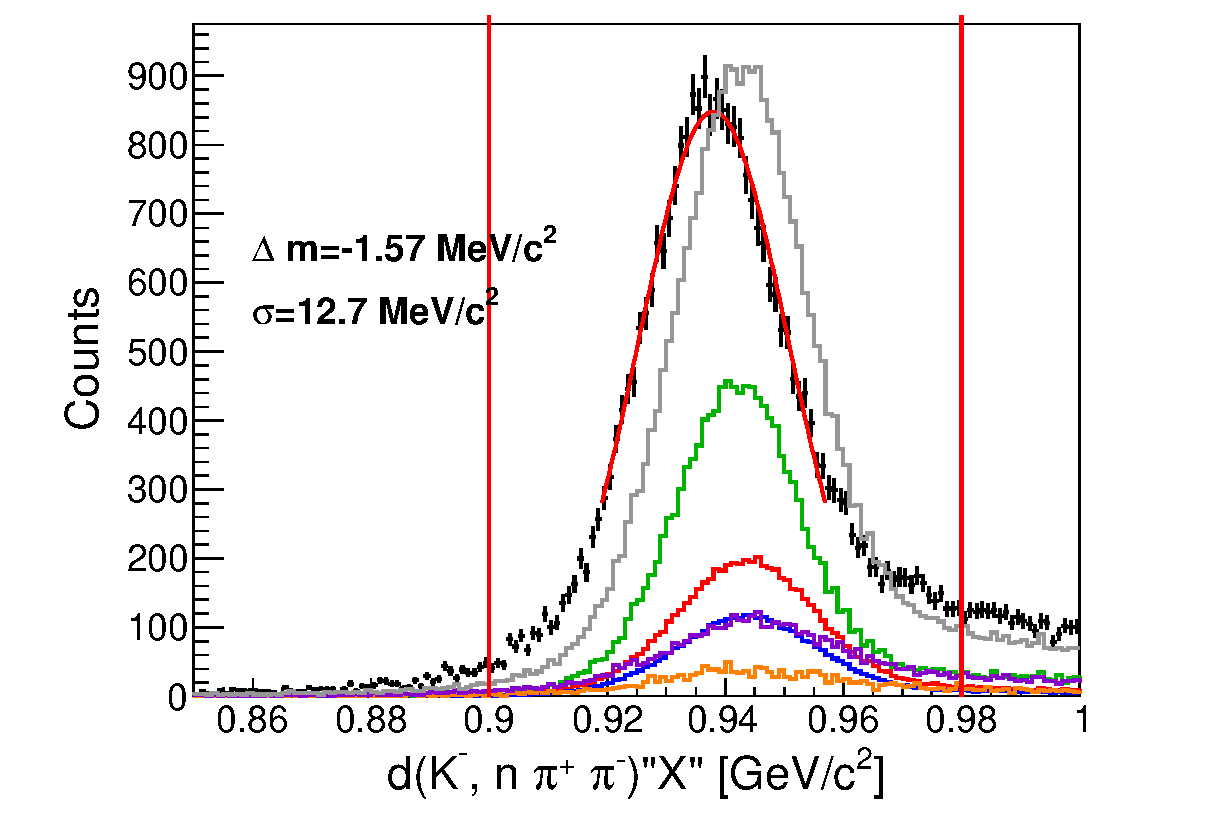
\includegraphics[width=3cm]{../pic/Run78/KN_ana_3sigma/fitKNpipi_MM_fitData.eps}\\
        MC fitting\\
        \includegraphics[width=3cm]{../pic/Run78/KN_ana_3sigma/fitKNpipi_MM_fitMC.eps}
      \end{figure}
    \end{minipage}
  \end{tabular}
\end{frame}
 
\begin{frame}{Invaraint mass by CDS}
  \begin{tabular}{cc}
    \begin{minipage}{0.5\hsize}
      \begin{figure}
        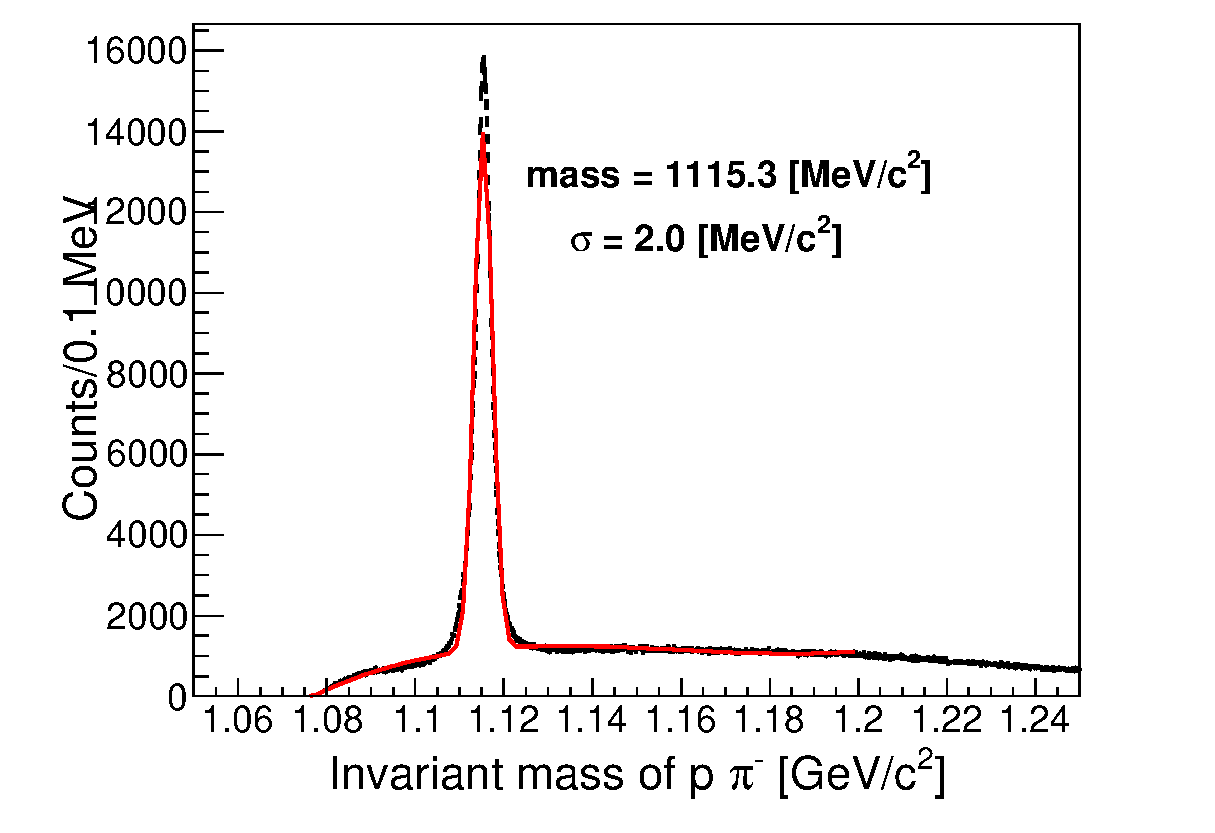
\includegraphics[width=5cm]{../pic/Run78/CDS/IM_ppim.eps}
      \end{figure}
    \end{minipage}

    \begin{minipage}{0.5\hsize}
      \begin{figure}
        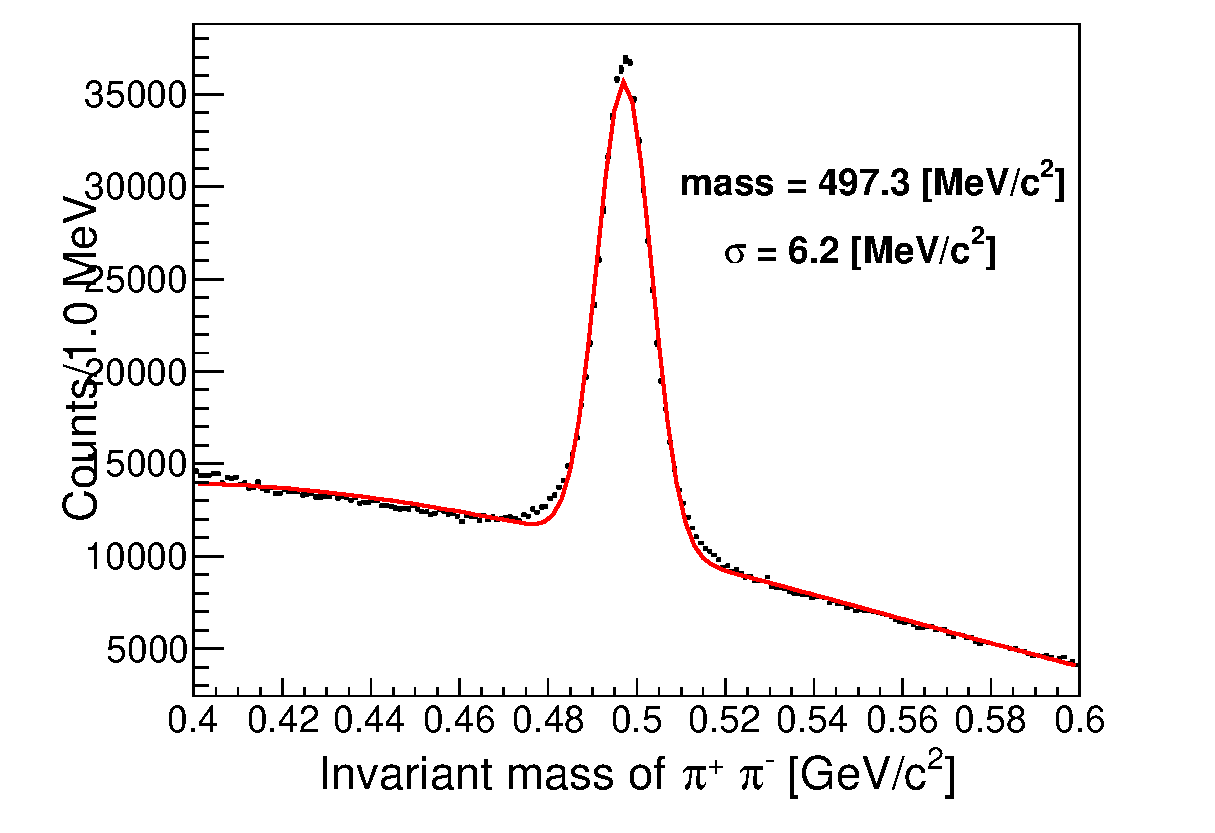
\includegraphics[width=5cm]{../pic/Run78/CDS/IM_pipi.eps}
      \end{figure}
    \end{minipage}
  \end{tabular}
\end{frame}

\begin{frame}{Template Fittig (All result summed) (NC $\sigma=170ps$)}
  $\pi^-\Sigma^+$ and $\pi^+ \Sigma^-$ modes were separated by fitting of $d(K^-, n \pi^{\pm})"\Sigma^{\mp}"$ .\\
  This fitting was performed bin-by-bin.
  
  \begin{figure}
    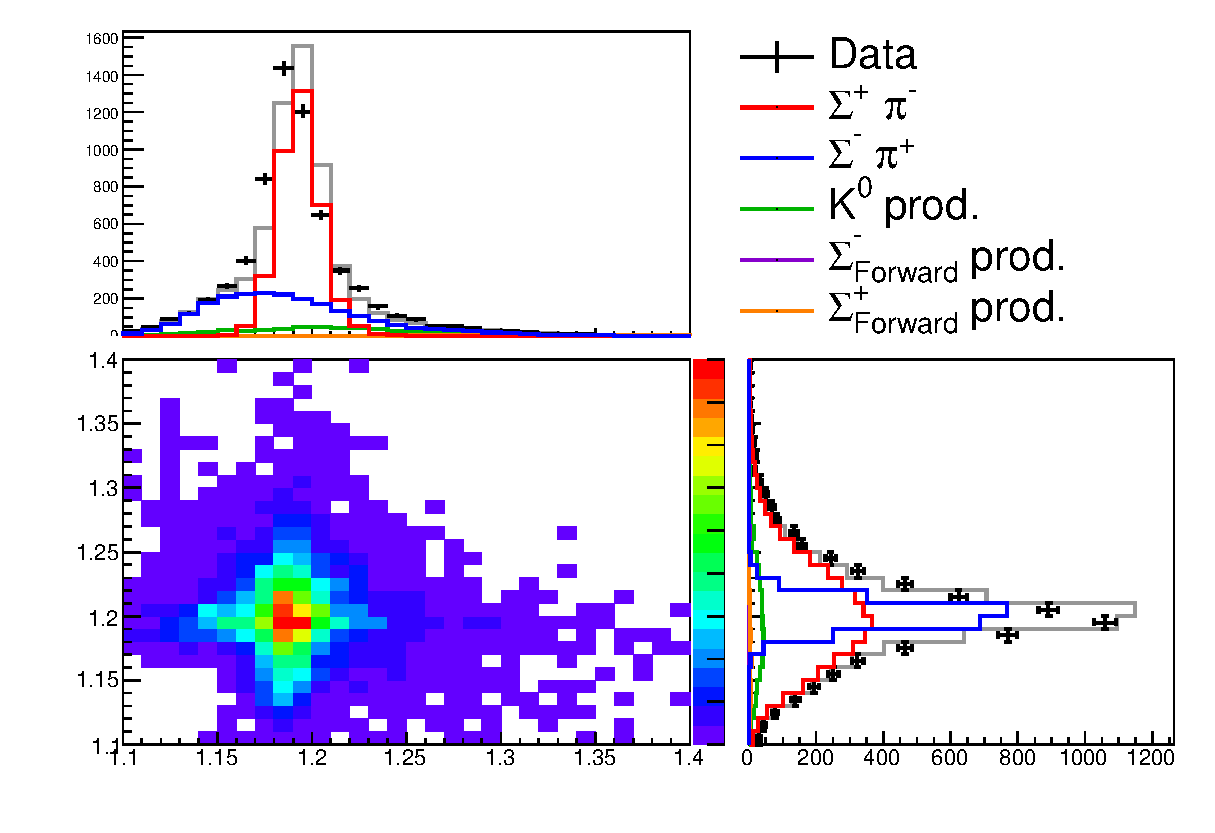
\includegraphics[width=6cm]{../pic/Run78/KN_ana_NC170_2sigma/KNpim_KNpip_MM.eps}
  \end{figure}
\end{frame}

\begin{frame}{$d(K^-, n \pi)"\Sigma"$ Fitting (NC $\sigma=150ps$)}
  \begin{tabular}{cc}
    \begin{minipage}{0.5\hsize}
      \begin{figure}
        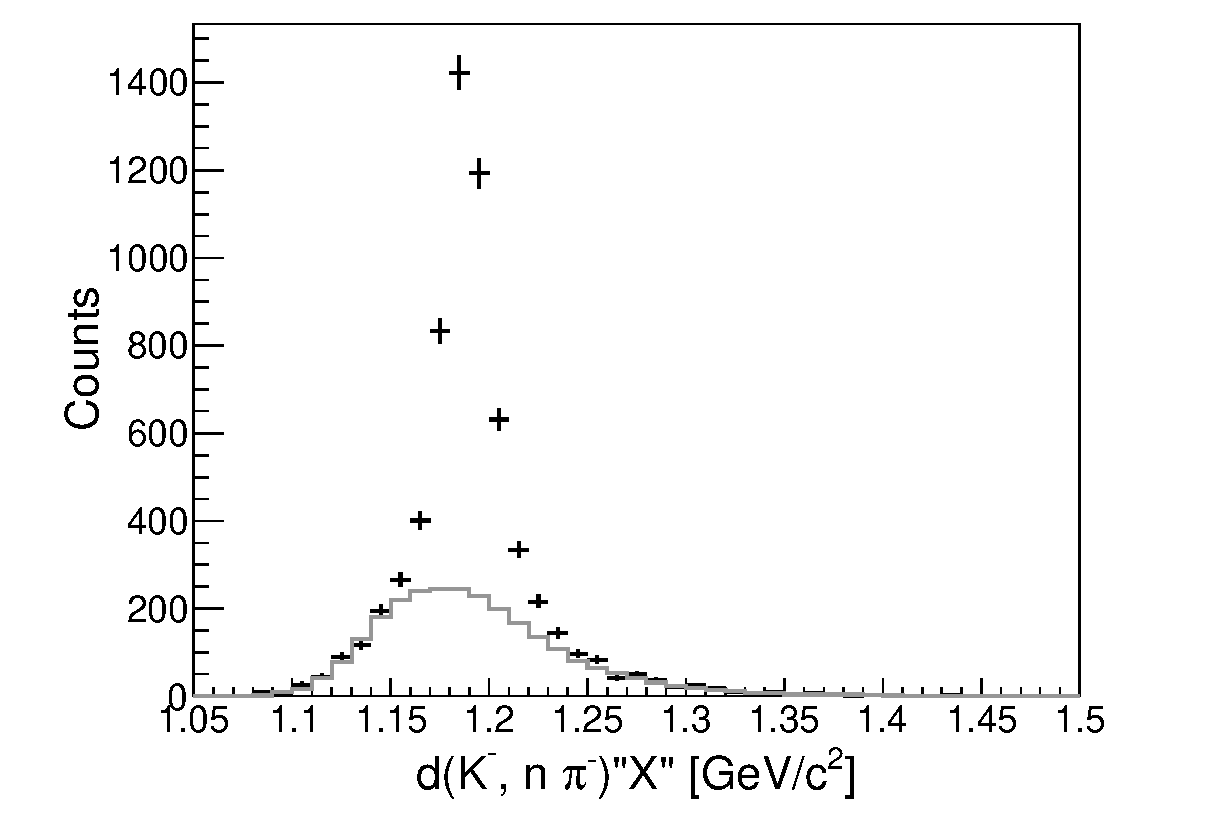
\includegraphics[width=3cm]{../pic/Run78/KN_ana_3sigma/fitKNpim_MM_data_wBG.eps}
      \end{figure}
    \end{minipage}

    \begin{minipage}{0.5\hsize}
      \begin{figure}
        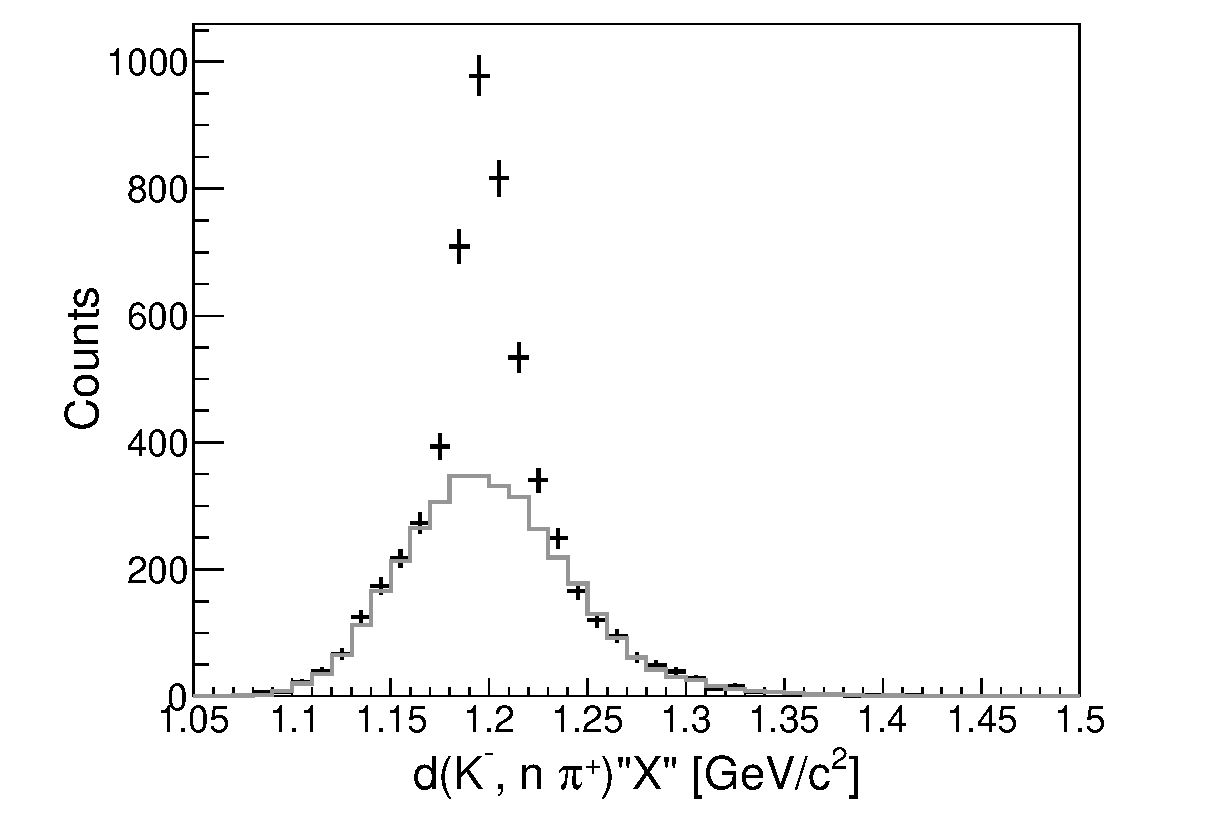
\includegraphics[width=3cm]{../pic/Run78/KN_ana_3sigma/fitKNpip_MM_data_wBG.eps}
      \end{figure}
    \end{minipage}
  \end{tabular}

  \begin{tabular}{cc}
    \begin{minipage}{0.5\hsize}
      \begin{figure}
        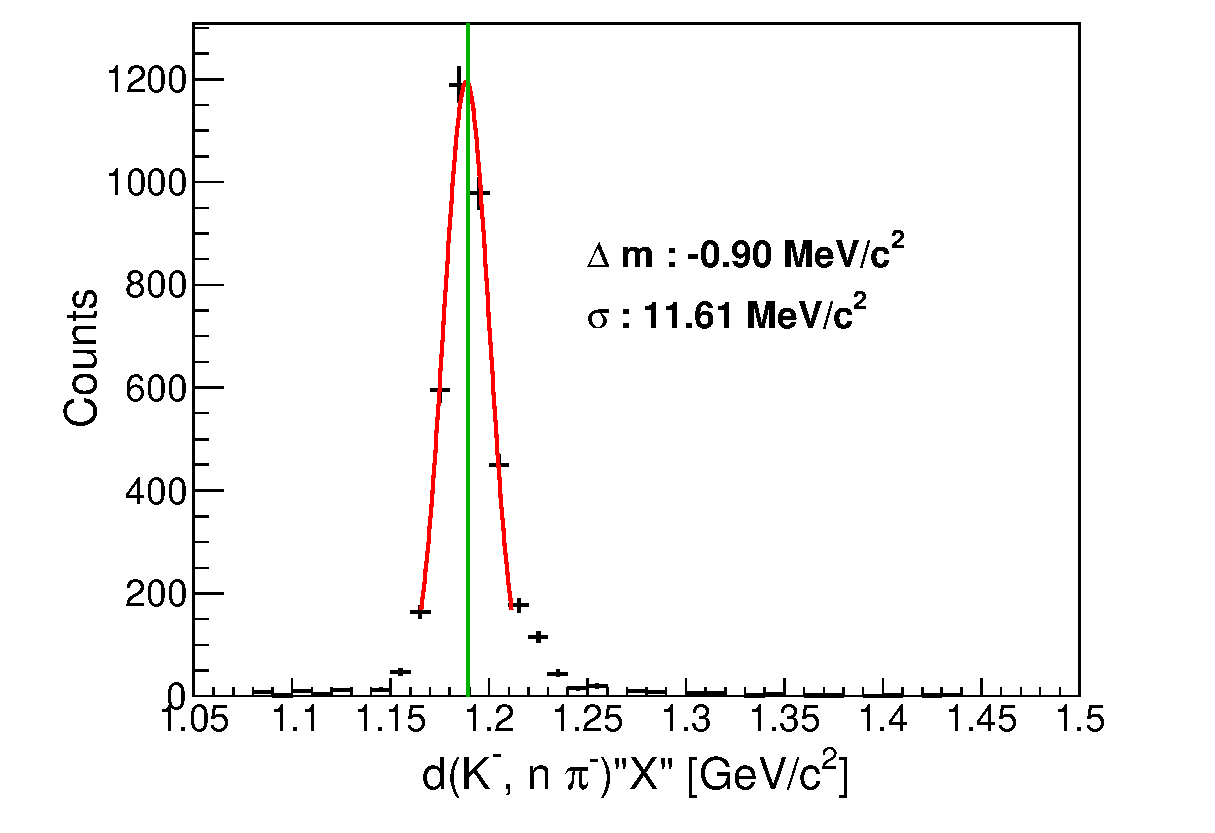
\includegraphics[width=3cm]{../pic/Run78/KN_ana_3sigma/fitKNpim_MM_data.eps}
      \end{figure}
    \end{minipage}

    \begin{minipage}{0.5\hsize}
      \begin{figure}
        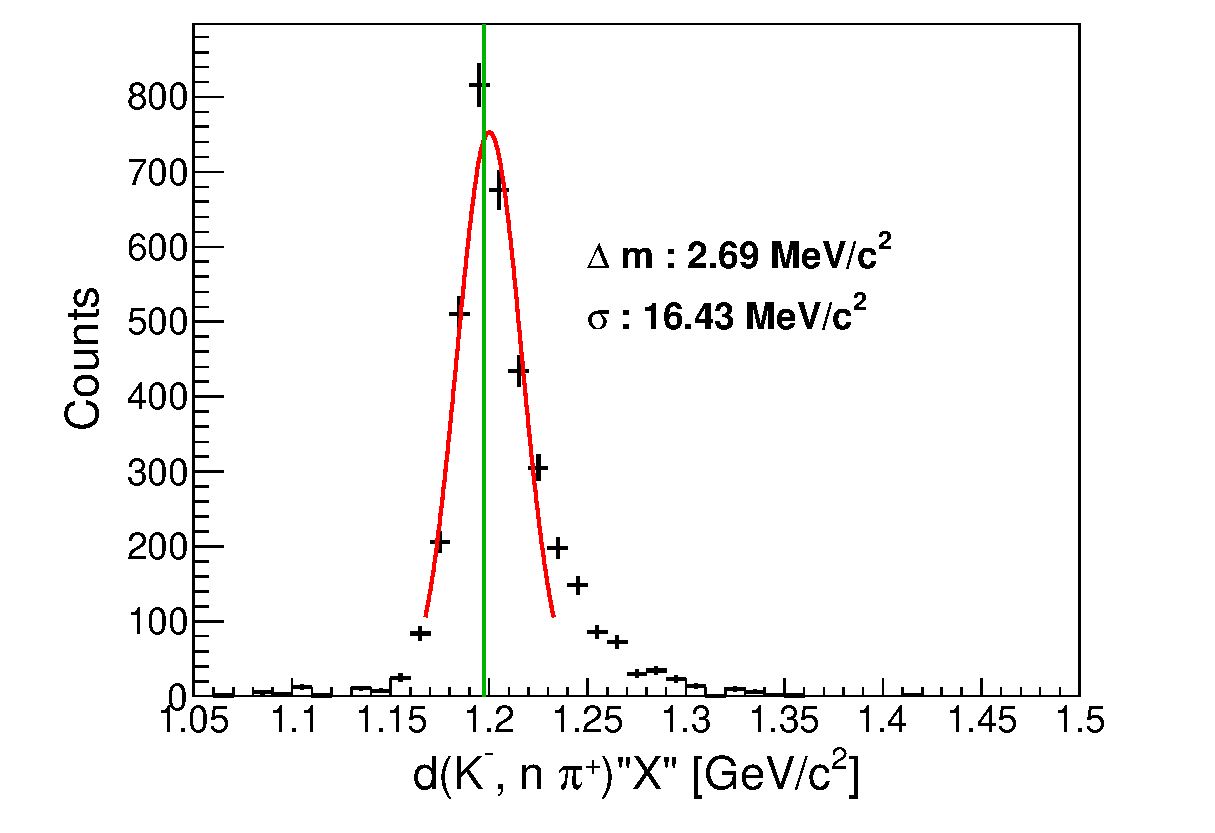
\includegraphics[width=3cm]{../pic/Run78/KN_ana_3sigma/fitKNpip_MM_data.eps}
      \end{figure}
    \end{minipage}
  \end{tabular}

  \begin{tabular}{cc}
    \begin{minipage}{0.5\hsize}
      \begin{figure}
        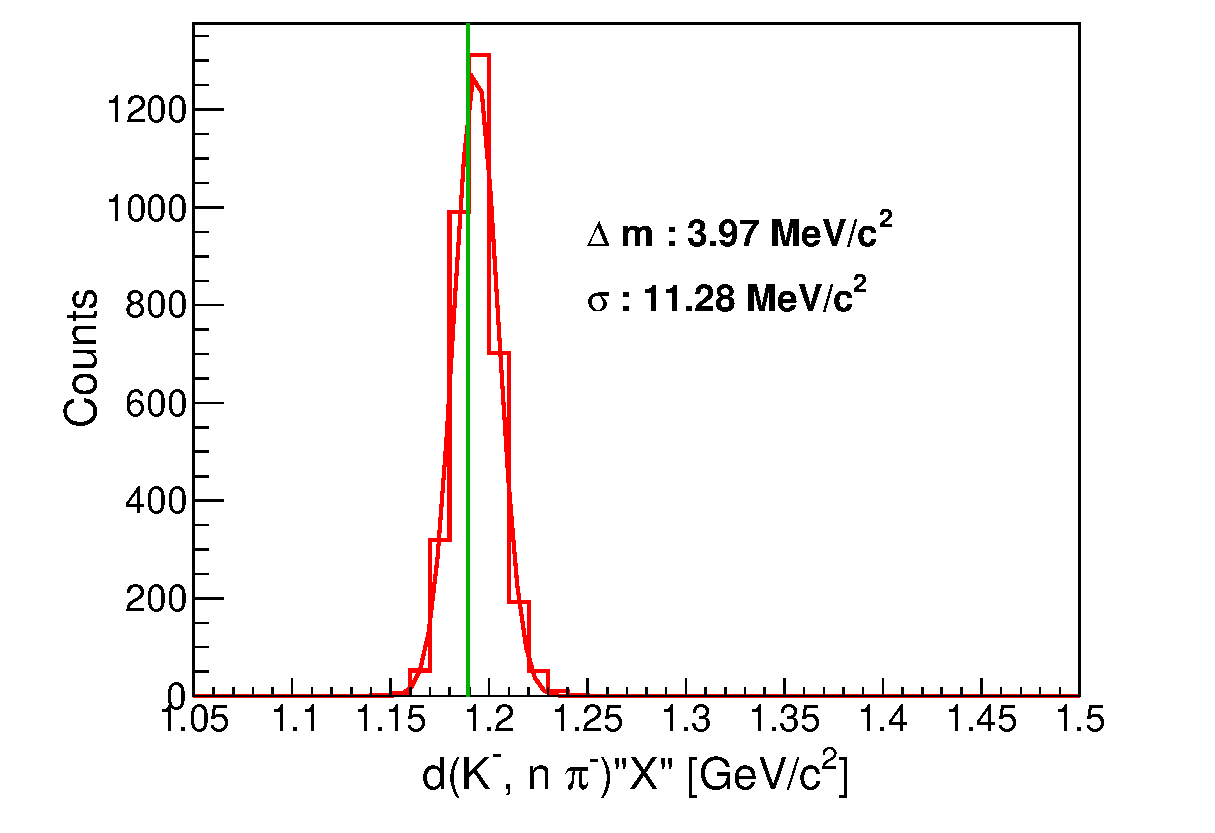
\includegraphics[width=3cm]{../pic/Run78/KN_ana_3sigma/fitKNpim_MM_MC.eps}
      \end{figure}
    \end{minipage}

    \begin{minipage}{0.5\hsize}
      \begin{figure}
        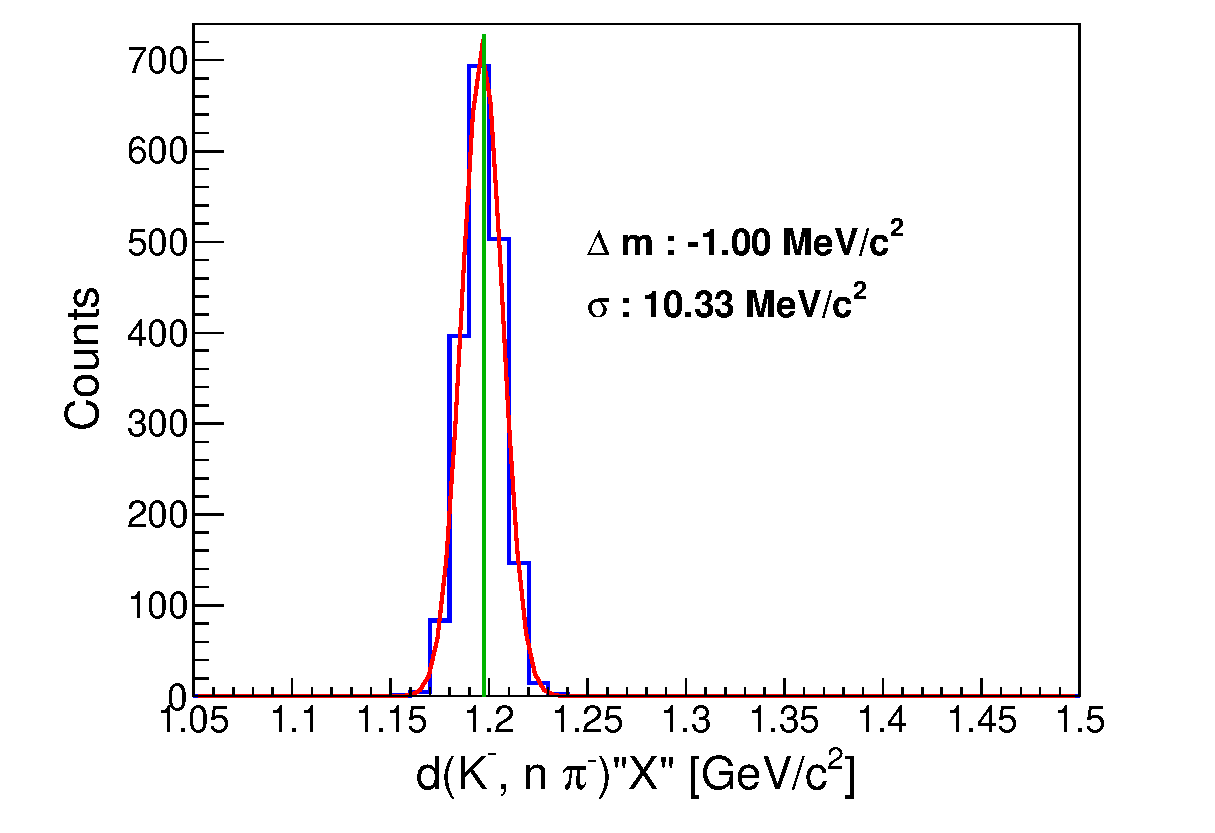
\includegraphics[width=3cm]{../pic/Run78/KN_ana_3sigma/fitKNpip_MM_MC.eps}
      \end{figure}
    \end{minipage}
  \end{tabular}
\end{frame}

\begin{frame}{$\ln(\Lambda)$}
  \begin{figure}
    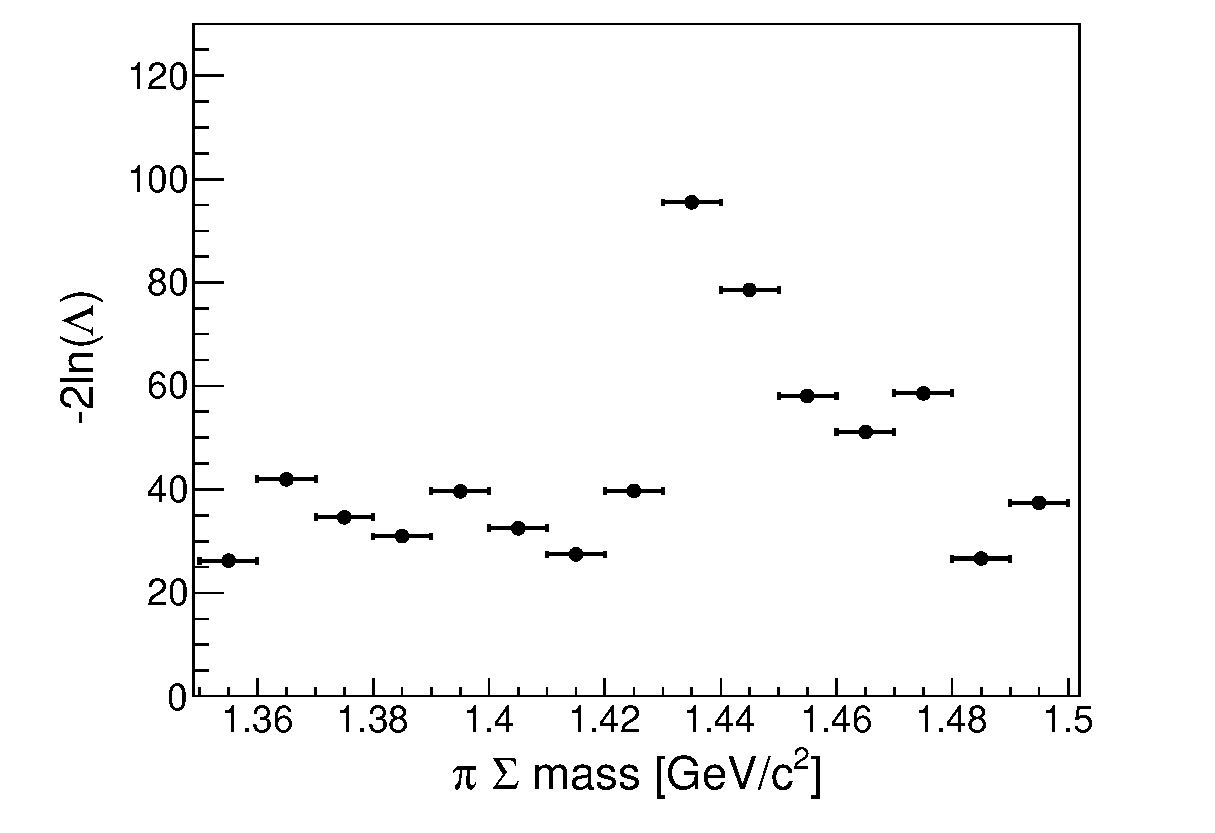
\includegraphics[width=10cm]{../pic/Run78/KN_ana_NC170_25sigma/Chi2.eps}
  \end{figure}
\end{frame}

\begin{frame}{Separated $\pi^{\pm}\Sigma^{\mp}$ Number}
  \begin{figure}
    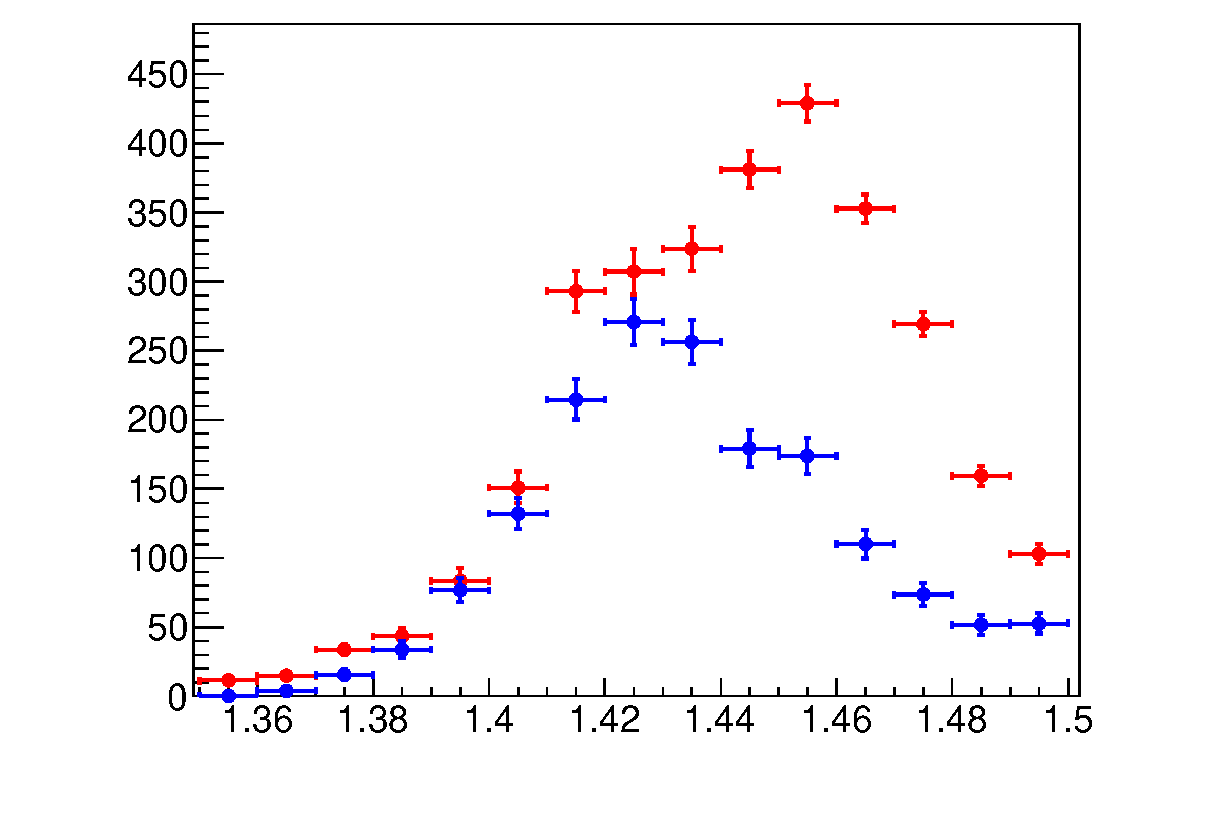
\includegraphics[width=8cm]{../pic/Run78/KN_ana_3sigma/piS_num.eps}
  \end{figure}
\end{frame}

\begin{frame}{Acceptance of $\pi^{\pm}\Sigma^{\mp}$}
  \begin{figure}
    \includegraphics[width=8cm]{../pic/Run78/KN_ana_3sigma/kn_acc.eps}
  \end{figure}
\end{frame}

\begin{frame}{$\pi^{\pm}\Sigma^{\mp}$ Cross Section}
  \begin{figure}
    \includegraphics[width=7cm]{../pic/Run78/KN_ana_3sigma/pimSp_pipSm_CS.eps}
  \end{figure}
\end{frame}

\begin{frame}{$\pi^{\pm}\Sigma^{\mp}$ Average Cross Section}
  \begin{figure}
    \includegraphics[width=7cm]{../pic/Run78/KN_ana_3sigma/Charge_ave_CS.eps}
  \end{figure}
\end{frame}

%% \input{KN_ana_NC170_2sigma/KNpi_MM/KNpi_MM_0}
\input{KN_ana_NC170_2sigma/KNpi_MM/KNpi_MM_1}
\input{KN_ana_NC170_2sigma/KNpi_MM/KNpi_MM_2}
\input{KN_ana_NC170_2sigma/KNpi_MM/KNpi_MM_3}
\input{KN_ana_NC170_2sigma/KNpi_MM/KNpi_MM_4}
\input{KN_ana_NC170_2sigma/KNpi_MM/KNpi_MM_5}
\input{KN_ana_NC170_2sigma/KNpi_MM/KNpi_MM_6}
\input{KN_ana_NC170_2sigma/KNpi_MM/KNpi_MM_7}
\input{KN_ana_NC170_2sigma/KNpi_MM/KNpi_MM_8}
\input{KN_ana_NC170_2sigma/KNpi_MM/KNpi_MM_9}
\input{KN_ana_NC170_2sigma/KNpi_MM/KNpi_MM_10}
\input{KN_ana_NC170_2sigma/KNpi_MM/KNpi_MM_11}
\input{KN_ana_NC170_2sigma/KNpi_MM/KNpi_MM_12}
\input{KN_ana_NC170_2sigma/KNpi_MM/KNpi_MM_13}
\input{KN_ana_NC170_2sigma/KNpi_MM/KNpi_MM_14}
\input{KN_ana_NC170_2sigma/KNpi_MM/KNpi_MM_15}
\input{KN_ana_NC170_2sigma/KNpi_MM/KNpi_MM_16}
\input{KN_ana_NC170_2sigma/KNpi_MM/KNpi_MM_17}
\input{KN_ana_NC170_2sigma/KNpi_MM/KNpi_MM_18}
\input{KN_ana_NC170_2sigma/KNpi_MM/KNpi_MM_19}
\input{KN_ana_NC170_2sigma/KNpi_MM/KNpi_MM_20}
\input{KN_ana_NC170_2sigma/KNpi_MM/KNpi_MM_21}
\input{KN_ana_NC170_2sigma/KNpi_MM/KNpi_MM_22}
\input{KN_ana_NC170_2sigma/KNpi_MM/KNpi_MM_23}
\input{KN_ana_NC170_2sigma/KNpi_MM/KNpi_MM_24}



%% \begin{frame}{Summary of error estimation}
  \begin{itemize}
  \item Difference of horizontal axis.
    $\rightarrow$ Estimation using $d(K^-, n \pi^+ \pi^-)"n"$, $d(K^-, n \pi^-)"\Sigma^+"$ and $d(K^-, n \pi^+)"\Sigma^-"$ peaks\\
    $\rightarrow$ Difference within 2$MeV/c^2$.
  \item Staticical error of $d(K^-, n \pi^+ \pi^-)"n"$ events.\\
    $\rightarrow$ $\sim 3.9\%$ in maximum bin.
  \item Systematic error of template fitting ($d(K^-, n \pi^{\mp})"\Sigma^{\pm}"$)\\
    \small
    $\rightarrow$ $d(K^-, n \pi^-)"\Sigma^+" \sim 4.8\%$ $d(K^-, n \pi^+)"\Sigma^-" \sim 8.6\%$ average$\sim 4.1\%$
  \item Scaling factor error
    \begin{table}
      \begin{tabular}{|c|c|c|}
        \hline
        item          & ratio & value$\pm$ error \\
        \hline
        Luminosity    & 2.6\%  & $(5.162 \pm 0.014)\times 10^3$ \\
        NC efficiency & 5.0\%  & $0.291 \pm 0.016$ \\
        \hline
        \hline
        intrinsic          &   & $ 0.317 \pm 0.016$ \\
        Overkill$_CVC/BVC$ &   & $ 0.919 \pm 0.007$ \\
        \hline
        \hline
        CDC efficiency & 0.4\% & $0.977 \pm 0.004$ \\
        \hline
        \hline
        Sum & 5.6\% & \\
        \hline
      \end{tabular}
    \end{table}
  \end{itemize}
  \tiny
  \centering
  \href{http://ag.riken.jp/J-PARC/inoue/kd_ana/all.pdf}
  {These analysis details in this link}
\end{frame}

\begin{frame}{$d(K^-, n K^0)"n"$  event}
  \tminipageTwo{
    \begin{figure}
      \includegraphics[width=3cm]{../pic/Run78/KN_ana_NC170_2sigma/KNpipi_MM_woFit.eps}
      \captionsetup{font=scriptsize}
      \caption{
        Event Sample : $d(K^-, n \pi^+ \pi^-)"n"$
      }
    \end{figure}
  }{
    \begin{figure} 
      \includegraphics[width=3cm]{../pic/Run78/KN_ana_NC170_2sigma/IM_pipi_select.eps}
      \captionsetup{font=scriptsize}
      \caption{
        \centering
        $K^0$ selection. \protect\linebreak
        Color plots indicates background events, \protect\linebreak
    7   which were estimated by template fittings.
%        $K^0$の選別、色線はp.\pageref{page:Fit_IM}のフィットで見積もられた。
%        バックグランドのイベントの分布を表す。
      }
    \end{figure}
  }
  \begin{tabular}{cc}
    \begin{minipage}{0.4\hsize}
      \begin{figure}
        \includegraphics[width=5cm]{../pic/Run78/QE/KN_MM_wK0_tag.eps}
      \end{figure}
    \end{minipage}
    \begin{minipage}{0.6\hsize}
      \centering
      \scriptsize
      Left figure shows $d(K^-, n K^0)"n"$ events spectrum.\\
      Color plots indicate background reaction.
%      左図は上右図によって$K^0$選別されたイベント\\
%      色線は他の反応からのバックグラウンド
    \end{minipage}
  \end{tabular}
\end{frame}

\begin{frame}{Acceptance distribution}
  %%  Reaction: $K^- d \rightarrow n_{forward} (K^0 n)$ $K^0 n$ mass : $1.45 \sim 1.8 [GeV/c^{2}]$\\
  \centering
  \begin{equation*}
    K^{-} d \rightarrow K^0 "n" n_{detected}  | m_{"n" K^{0}} : \mbox{from threshold} \sim 1.8 GeV/c^2
  \end{equation*}
  (Analyzed event)/(Generated event)
  \begin{figure}
    $A(\cos\theta_{K^0}, p_{K^0})$\\
    \includegraphics[width=7cm]{../pic/Run78/QE/K0_cos_mom_acc.eps}
  \end{figure}
\end{frame}

\begin{frame}{$K^0 cos\theta$ vs mom  {\bf Data}}
  \begin{tabular}{cc}
    \begin{minipage}{0.5\hsize}
      \begin{figure}
        Raw\\
        \includegraphics[width=6cm]{../pic/Run78/QE/K0_cos_mom_data.eps}
      \end{figure}
    \end{minipage}

    \begin{minipage}{0.5\hsize}
      \begin{figure}
        $Data(\cos_{K^0}, p_{K^0}))/A(\cos\theta_{K^0}, p_{K^0})$\\
%%        Accpectance corrected\\
        \includegraphics[width=6cm]{../pic/Run78/QE/K0_cos_mom_data_corr.eps}
      \end{figure}
    \end{minipage}
  \end{tabular}
  
  \centering

  Acceptance was presented at page.4
  
\end{frame}

\begin{frame}{$K^0 cos\theta$ vs mom {\bf Background}}
  \begin{tabular}{cc}
    \begin{minipage}{0.5\hsize}
      \begin{figure}
        BG sum w/o acc corr.\\
        \includegraphics[width=4.5cm]{../pic/Run78/QE/K0_cos_mom_BG.eps}
      \end{figure}
    \end{minipage}

    \begin{minipage}{0.5\hsize}
      \begin{figure}
        BG sum w/ acc corr.\\
        \includegraphics[width=4.5cm]{../pic/Run78/QE/K0_cos_mom_sum_corr.eps}
      \end{figure}
    \end{minipage}
  \end{tabular}
  
  \centering
  These figures indicate each processes.
  
  \begin{tabular}{cc}
    \begin{minipage}{0.5\hsize}
      \begin{tabular}{cc}
        \begin{minipage}{0.5\hsize}
          \begin{figure}
            { \scriptsize 
              $(\pi^+\Sigma^-)_{backward}$
            }
            \includegraphics[width=2cm]{../pic/Run78/QE/K0_cos_mom_pimSp.eps}
          \end{figure}
        \end{minipage}
        
        \begin{minipage}{0.5\hsize}
          \begin{figure}
            { \scriptsize 
              $(\pi^+\Sigma^-)_{backward}$
            }
            \includegraphics[width=2cm]{../pic/Run78/QE/K0_cos_mom_pipSm.eps}
          \end{figure}
        \end{minipage}
      \end{tabular}

      \begin{tabular}{cc}
        \begin{minipage}{0.5\hsize}
          \begin{figure}
            { \scriptsize 
              $\pi^+\Sigma^-_{forward}$
            }
            \includegraphics[width=2cm]{../pic/Run78/QE/K0_cos_mom_Sm.eps}
          \end{figure}
        \end{minipage}
        
        \begin{minipage}{0.5\hsize}
          \begin{figure}
            { \scriptsize 
              $\pi^-\Sigma^+_{forward}$
            }
            \includegraphics[width=2cm]{../pic/Run78/QE/K0_cos_mom_Sp.eps}
          \end{figure}
        \end{minipage}
      \end{tabular}
    \end{minipage}

    \begin{minipage}{0.5\hsize}
      \begin{tabular}{cc}
        \begin{minipage}{0.5\hsize}
          \begin{figure}
            { \scriptsize 
              $(\pi^+\Sigma^-)_{backward}$
            }
            \includegraphics[width=2cm]{../pic/Run78/QE/K0_cos_mom_pimSp_corr.eps}
          \end{figure}
        \end{minipage}
        
        \begin{minipage}{0.5\hsize}
          \begin{figure}
            { \scriptsize 
              $(\pi^+\Sigma^-)_{backward}$
            }
            \includegraphics[width=2cm]{../pic/Run78/QE/K0_cos_mom_pipSm_corr.eps}
          \end{figure}
        \end{minipage}
      \end{tabular}

      \begin{tabular}{cc}
        \begin{minipage}{0.5\hsize}
          \begin{figure}
            { \scriptsize 
              $\pi^+\Sigma^-_{forward}$
            }
            \includegraphics[width=2cm]{../pic/Run78/QE/K0_cos_mom_Sm_corr.eps}
          \end{figure}
        \end{minipage}
        
        \begin{minipage}{0.5\hsize}
          \begin{figure}
            { \scriptsize 
              $\pi^-\Sigma^+_{forward}$
            }
            \includegraphics[width=2cm]{../pic/Run78/QE/K0_cos_mom_Sp_corr.eps}
          \end{figure}
        \end{minipage}
      \end{tabular}
    \end{minipage}
  \end{tabular}
\end{frame}

%% \begin{frame}{Background subtraction}
  \begin{tabular}{cc}
    \begin{minipage}{0.5\hsize}
      \begin{figure}
        BG ratio (BG/Data)
        \includegraphics[width=4.5cm]{../pic/Run78/QE/K0_cos_mom_BG_ratio.eps}
      \end{figure}
    \end{minipage}
    
    \begin{minipage}{0.5\hsize}
      Acceptance was estimated using\\
      $K^- d \rightarrow (K^0 n) n_{forward}$\\ (($K^0$ n) : 1.436$\sim$ 1.8 $[Gev/c^2]$)\\
      
      
    \end{minipage}
  \end{tabular}

  \begin{tabular}{cc}
    \begin{minipage}{0.5\hsize}
      \begin{figure}
        Acceptance
        \includegraphics[width=4.5cm]{../pic/Run78/QE/K0_cos_mom_acc.eps}
      \end{figure}
    \end{minipage}
    
    \begin{minipage}{0.5\hsize}
      \begin{figure}
        Acceptance w/ BG ratio
        \includegraphics[width=4.5cm]{../pic/Run78/QE/K0_cos_mom_acc_wBG.eps}
      \end{figure}
    \end{minipage}
  \end{tabular}      
\end{frame}

\begin{frame}{$d(K^-, n)"n K^0"$ (Acc corrected)}
  \begin{figure}
    $N(d(K^-, n)"X") / Acc(\cos\theta_{K^0}, mom_{K^0})$\\
    \includegraphics[width=8cm]{../pic/Run78/QE/K0_spec_wBG.eps}
  \end{figure}
  \centering
  Background processes were adopted same analysis.
\end{frame}

\begin{frame}{Cross Section of $d(K^-, n)"n K^0"$}
  \begin{figure}
    \includegraphics[width=8cm]{../pic/Run78/QE/K0_CS.eps}
  \end{figure}
  \centering
  Box indicates staticial errors.
%%  BG was subtracted.
\end{frame}


\chapter{Conclusion}
We measured $d(K^, N)"\pi\Sigma"$ reaction with $1GeV$/c $K^-$ beam at K1.8BR beamline of the hadron hoall in the J-PARC as the J-PARC E31 experiment.
We measured forward scattering scattering nucleon using the NC and PC.
Simultaneously,	decayed	particles are detected by the CDS surrounding the	liquid-$D_2$ target to identified final	state.
We identify $K^- d \rightarrow n \pi^+ \pi^- n$ final state and removed $K^0$ and forward-$\Sigma^{\pm}$ production, in which forward-$\Sigma^{\pm}$ means forward neutron decayed from $\Sigma^{\pm}$.
And, we obtain $d(K^-, n)"\pi^{\mp}\Sigma^{\pm}"$, which decomposed to $\pi^-\Sigma^+$ and $\pi^+\Sigma^-$ from missing mass of $d(K^-, n \pi^{\mp})"\Sigma^{\pm}"$.
We identify $\pi^-\Sigma^0$ final state from identify $d(K^-, p \pi^-)"\Sigma^0"$ and $d(K^-, p \pi^- \pi^-)"p"$.
At the result, We obtained \pimSp, \pipSm and \pimSz cross sections from the missing mass of the $d(K^, N)$ missing mass.

This reaction is considered as the 2-step reaction of $K^-N\rightarrow \bar{K}N$ scattering and $\bar{K}N \rightarrow \pi \Sigma$ scattering.
1-step reaction has large energy $\sim 2.05 GeV/$c and 2-step can allow to occur $\bar{K}N \rightarrow \pi \Sigma$  below the $\bar{K}N$ threshold.
Large energy 1-step reaction restricts the contamination from 1-step reaction in which a nucleon	emitted	as the spectator around the $\bar{K}N$ threshold.
Because the recoiled $\bar{K}$ has low momentum $\sim 0.25 GeV$/c around the $\bar{K}N$ threshold, the S-wave scattering is dominant in 2-step $\bar{K}N \rightarrow \pi \Sigma$ scattering,
which is confirmed from our data not to see obvious peak around the $\Sigma(1385)$ and $\Lambda(1520)$, which are P-wave and D-wave.
We can understand the reaction is the above the mechanism from the matching our data and theoretical calculations which adopts or covers around high energy $\bar{K}N$ scattering region around 1-step.

We decompose about the isospin $I=0$, $I=1$ and these interference term about 2-step scattering. %%ToDo スペクトルの説明
The so-called model.B is not matched spectra shape of $\pi^-\Sigma^+$ and $\pi^+ \Sigma^-$, especially below the $\bar{K}N$ threshold,
because this has large width of higher pole.
On the other hand, in model.B, obtained spectra are reproduced to change all $I=0$, $I=1$ and these interference term.
That means that $I=0$ component is important, but $I=1$ component is also important even though the component does not have pole in the region of interest.
That means that $I=0$ component is important, but $I=1$ component is also important even though the component does not have pole in the region of interest.
Above the threshold, $I=0$ $\pi^-\Sigma^0$ has large cross section and the interference term between $I=0$ and $I=1$ also appear as the difference of $\pi^-\Sigma^+$ and $\pi^+\Sigma^-$.
So, interference term is necessary to explain the these three spectra.

We obtain $\pi^-\Sigma^+$, $\pi^+\Sigma^-$ and $\pi^-\Sigma^0$ spectra via the $d(K^-, N)$ reaction,
which is considered 2-step reaction of $K^-N\rightarrow \bar{K}N$ and $\bar{K}N \rightarrow \pi\Sigma$.
These spectra provide all information to determine that $I=0$, $I=1$ and these interference term of $\bar{K}N \rightarrow \pi\Sigma$ scattering around the $\bar{K}N$ threshold.




% And we compare with the theoretical calculation of the dynamical-coupled framework, which can comprehensively treat 1-step and 2-step scattering.







%% \begin{frame}{$K^0 cos\theta$ vs mom {\bf BG subtracted}}
  \begin{tabular}{cc}
    \begin{minipage}{0.5\hsize}
      \begin{figure}
        Raw \\
        \includegraphics[width=6cm]{../pic/Run78//QE//K0_cos_mom_BGsub.eps}
      \end{figure}
    \end{minipage}

    \begin{minipage}{0.5\hsize}
      \begin{figure}
        Acceptanfe corrected.\\
        \includegraphics[width=6cm]{../pic/Run78//QE//K0_cos_mom_BGsub_corr.eps}
      \end{figure}
    \end{minipage}
  \end{tabular}    
\end{frame}

%% \begin{frame}{$K^0$ $\cos\theta$ vs mom ($d(K^-, n)"X"$ dependence)}
  \begin{tabular}{ccc}
    \begin{minipage}{0.33\hsize}
      \begin{figure}
        
        { \tiny $d(K^-, n)$ : 1.45 $\sim$ 1.50 $[GeV/c^2]$  }          
        \includegraphics[width=3cm]{../pic/Run78/QE/K0_cos_mom_145_150.eps}
      \end{figure}
    \end{minipage}

    \begin{minipage}{0.33\hsize}
      \begin{figure}

        { \tiny $d(K^-, n)$ : 1.50 $\sim$ 1.55 $[GeV/c^2]$  }          
        \includegraphics[width=3cm]{../pic/Run78/QE/K0_cos_mom_150_155.eps}
      \end{figure}
    \end{minipage}

    \begin{minipage}{0.33\hsize}
      \begin{figure}

        { \tiny $d(K^-, n)$ : 1.55 $\sim$ 1.60 $[GeV/c^2]$  }
        \includegraphics[width=3cm]{../pic/Run78/QE/K0_cos_mom_155_160.eps}
      \end{figure}
    \end{minipage}
  \end{tabular}

  \begin{tabular}{ccc}
    \begin{minipage}{0.33\hsize}
      \begin{figure}
        
        { \tiny $d(K^-, n)$ : 1.60 $\sim$ 1.65 $[GeV/c^2]$  }          
        \includegraphics[width=3cm]{../pic/Run78/QE/K0_cos_mom_160_165.eps}
      \end{figure}
    \end{minipage}

    \begin{minipage}{0.33\hsize}
      \begin{figure}

        { \tiny $d(K^-, n)$ : 1.65 $\sim$ 1.70 $[GeV/c^2]$  }          
        \includegraphics[width=3cm]{../pic/Run78/QE/K0_cos_mom_165_170.eps}
      \end{figure}
    \end{minipage}

    \begin{minipage}{0.33\hsize}
      \begin{figure}

        { \tiny $d(K^-, n)$ : 1.70 $\sim$ 1.75 $[GeV/c^2]$  }
        \includegraphics[width=3cm]{../pic/Run78/QE/K0_cos_mom_170_175.eps}
      \end{figure}
    \end{minipage}
  \end{tabular}

  \begin{tabular}{cc}
    \begin{minipage}{0.33\hsize}
      \begin{figure}
        
        { \tiny $d(K^-, n)$ : 175 $\sim$ 1.80 $[GeV/c^2]$  }          
        \includegraphics[width=3cm]{../pic/Run78/QE/K0_cos_mom_175_180.eps}
      \end{figure}
    \end{minipage}

    \begin{minipage}{0.66\hsize}

    \end{minipage}
  \end{tabular}
\end{frame}



\begin{frame}


  Back up
\end{frame}



\begin{frame}{NC dE higher order correction}
  \begin{tabular}{cc}
    \begin{minipage}{0.5\hsize}
      \begin{figure}
        Before corr.
        \includegraphics[width=5cm]{../pic/Run78/calib/NCdE_KNpipi_MM.eps}
      \end{figure}
    \end{minipage}

    \begin{minipage}{0.5\hsize}
      \begin{figure}
        After corr.
        \includegraphics[width=5cm]{../pic/Run78/calib/NCdE_KNpipi_MM_mod.eps}
      \end{figure}
    \end{minipage}
  \end{tabular}

  \begin{tabular}{cc}
    \begin{minipage}{0.5\hsize}
      \begin{figure}
        \includegraphics[width=5cm]{../pic/Run78/calib/NCdE_delta_p.eps}
      \end{figure}
    \end{minipage}

    \begin{minipage}{0.5\hsize}
      \begin{figure}
        \includegraphics[width=5cm]{../pic/Run78/calib/NCdE_delta_p_mod.eps}
      \end{figure}
    \end{minipage}
  \end{tabular}
\end{frame}

\begin{frame}{Spectrum diff. by NC dE higher order corr.}
  \begin{tabular}{cc}
    \begin{minipage}{0.5\hsize}
      \hspace{3mm} Before \\
      \hspace{3mm} \color{red} After
    \end{minipage}

    \begin{minipage}{0.5\hsize}
      \begin{figure}
        \includegraphics[width=5cm]{../pic/Run78/calib_chk/KNpipi_MM.eps}
      \end{figure}
    \end{minipage}
  \end{tabular}
  
  \begin{tabular}{cc}
    \begin{minipage}{0.5\hsize}
      \begin{figure}
        \includegraphics[width=5cm]{../pic/Run78/calib_chk/KN_MM_pipi_wK0.eps}
      \end{figure}
    \end{minipage}

    \begin{minipage}{0.5\hsize}
      \begin{figure}
        \includegraphics[width=5cm]{../pic/Run78/calib_chk/KN_MM_pipi_woAll.eps}
      \end{figure}
    \end{minipage}
  \end{tabular}
\end{frame}


\end{document}

\usepackage{ulem} 
\usepackage[abs]{overpic}
\usepackage{tikz}
\usepackage{tikz-feynhand}

\usepackage[labelformat=empty,labelsep=none]{caption} % figure のキャプション Figure: を消去





\usetheme{Madrid}

\title{$d(K^-, N)"\pi Y"$ Analysis}
\subtitle{Figures for PRL}
\author{Kentaro Inoue}
\date{\today}

\begin{document}
\maketitle

\begin{frame}{Current figures}
  \begin{tabular}{ccc}
    \begin{minipage}{0.33\hsize}
      \includegraphics[width=4cm]{../pic/letter/KNpim_MM.eps}
    \end{minipage}
    
    \begin{minipage}{0.33\hsize}
      \includegraphics[width=4cm]{../pic/letter/KNpip_MM.eps}
    \end{minipage}
    
    \begin{minipage}{0.33\hsize}
      \includegraphics[width=4cm]{../pic/letter/IM_ppim.eps}
    \end{minipage}
  \end{tabular}
  
  \begin{tabular}{ccc}
    \begin{minipage}{0.33\hsize}
      \includegraphics[width=4cm]{../pic/letter/KNLpi_MM.eps}
    \end{minipage}
    
    \begin{minipage}{0.33\hsize}
      \includegraphics[width=4cm]{../pic/letter/KPpim_MM_2D.eps}
    \end{minipage}
    
    \begin{minipage}{0.33\hsize}
      \includegraphics[width=4cm]{../pic/letter/KPpimpim_MM.eps}
    \end{minipage}
  \end{tabular}
\end{frame}

\end{document}
